% Dokumen penjelasan workspace Flame in Freefall.
% Kompilasi (dua kali, supaya daftar isi dan rujukan terisi):
%   cd docs/laporan && pdflatex workspace.tex && pdflatex workspace.tex
% Angka di % Dihasilkan oleh scripts/workspace_inventory.py. Jangan disunting tangan.
\newcommand{\psiListed}{16.372}
\newcommand{\psiOnDisk}{10.184}
\newcommand{\psiOnDiskGB}{23,0 GB}
\newcommand{\psiInv}{24}
\newcommand{\psiSkippedSel}{6.157}
\newcommand{\psiTooLarge}{27}
\newcommand{\psiFailed}{0}
\newcommand{\psiExtra}{0}
\newcommand{\ntrsPdf}{512}
\newcommand{\ntrsTxt}{513}
\newcommand{\ntrsCit}{695}
\newcommand{\ntrsOff}{84}
\newcommand{\doiPdf}{64}
\newcommand{\nTests}{1.990}
\newcommand{\nTestRows}{1.871}
\newcommand{\nCampaign}{119}
\newcommand{\nInvGold}{24}
\newcommand{\nPub}{352}
\newcommand{\nPapersNtrs}{695}
\newcommand{\nPapersDoi}{295}
\newcommand{\nChunks}{7.688}
\newcommand{\nTables}{22}
\newcommand{\bEntity}{2.647}
\newcommand{\bArtifact}{1.036}
\newcommand{\bMeas}{18.888}
\newcommand{\bLink}{19.686}
\newcommand{\bRule}{6}
\newcommand{\bRuleHit}{1.245}
\newcommand{\bCard}{6}
\newcommand{\tierDerivedAuto}{5.494}
\newcommand{\tierModelPrediction}{1.222}
\newcommand{\tierNasaCalibrated}{2.829}
\newcommand{\tierNasaTable}{9.339}
\newcommand{\tierPaperClaim}{4}
\newcommand{\arsipFiles}{42}
\newcommand{\arsipSize}{252,7 MB}
\newcommand{\nFiles}{477}
\newcommand{\nScripts}{34}
 dan tabel di data/*.tex dihasilkan oleh
%   py -3 scripts/workspace_inventory.py
% Jalankan skrip itu dulu setiap kali data berubah.
\documentclass[11pt,a4paper]{report}
\usepackage[T1]{fontenc}
\usepackage[utf8]{inputenc}
\usepackage[indonesian]{babel}
\usepackage{lmodern}
\usepackage{microtype}
\usepackage[margin=2.3cm]{geometry}
\usepackage{booktabs,longtable,array,tabularx,multirow}
\usepackage{xcolor,graphicx,enumitem,caption,float}
\usepackage{amsmath}
\usepackage{tikz}
\usetikzlibrary{arrows.meta,positioning,fit,calc}
\usepackage{fancyhdr}
\usepackage{titlesec}
\usepackage[hidelinks]{hyperref}
\usepackage{url}

\graphicspath{{gambar/}}
% Dihasilkan oleh scripts/workspace_inventory.py. Jangan disunting tangan.
\newcommand{\psiListed}{16.372}
\newcommand{\psiOnDisk}{10.184}
\newcommand{\psiOnDiskGB}{23,0 GB}
\newcommand{\psiInv}{24}
\newcommand{\psiSkippedSel}{6.157}
\newcommand{\psiTooLarge}{27}
\newcommand{\psiFailed}{0}
\newcommand{\psiExtra}{0}
\newcommand{\ntrsPdf}{512}
\newcommand{\ntrsTxt}{513}
\newcommand{\ntrsCit}{695}
\newcommand{\ntrsOff}{84}
\newcommand{\doiPdf}{64}
\newcommand{\nTests}{1.990}
\newcommand{\nTestRows}{1.871}
\newcommand{\nCampaign}{119}
\newcommand{\nInvGold}{24}
\newcommand{\nPub}{352}
\newcommand{\nPapersNtrs}{695}
\newcommand{\nPapersDoi}{295}
\newcommand{\nChunks}{7.688}
\newcommand{\nTables}{22}
\newcommand{\bEntity}{2.647}
\newcommand{\bArtifact}{1.036}
\newcommand{\bMeas}{18.888}
\newcommand{\bLink}{19.686}
\newcommand{\bRule}{6}
\newcommand{\bRuleHit}{1.245}
\newcommand{\bCard}{6}
\newcommand{\tierDerivedAuto}{5.494}
\newcommand{\tierModelPrediction}{1.222}
\newcommand{\tierNasaCalibrated}{2.829}
\newcommand{\tierNasaTable}{9.339}
\newcommand{\tierPaperClaim}{4}
\newcommand{\arsipFiles}{42}
\newcommand{\arsipSize}{252,7 MB}
\newcommand{\nFiles}{477}
\newcommand{\nScripts}{34}


% ---- gaya
\definecolor{biru}{HTML}{2A78D6}
\definecolor{oranye}{HTML}{EB6834}
\definecolor{tinta2}{HTML}{52514E}
\definecolor{garis}{HTML}{C3C2B7}
\definecolor{kotak}{HTML}{F3F2EF}
\titleformat{\chapter}[display]{\normalfont\bfseries\color{black}}{\large\color{tinta2}Bab \thechapter}{4pt}{\LARGE}
\titlespacing*{\chapter}{0pt}{-10pt}{18pt}
\setlength{\parskip}{4pt}
\setlength{\parindent}{0pt}
\setlist{itemsep=2pt,topsep=3pt}
\captionsetup{font=small,labelfont=bf}
\pagestyle{fancy}\fancyhf{}
\fancyhead[L]{\small\color{tinta2}Flame in Freefall: penjelasan workspace}
\fancyhead[R]{\small\color{tinta2}\leftmark}
\fancyfoot[C]{\small\thepage}
\renewcommand{\headrulewidth}{0.3pt}

% ---- makro
\urlstyle{tt}
\makeatletter\g@addto@macro{\UrlBreaks}{\do\_\do\-}\makeatother
\newcommand{\berkas}{\path}                     % nama berkas & folder
\newcommand{\Od}{O\textsubscript{2}}
\newcommand{\COd}{CO\textsubscript{2}}
\newcommand{\Nd}{N\textsubscript{2}}
\newcommand{\asing}[1]{\textit{#1}}             % istilah asing, dimiringkan pada pemakaian pertama
\newcommand{\tier}[1]{\textsf{\small #1}}
\newcommand{\catatan}[2]{\par\smallskip\noindent\colorbox{kotak}{\begin{minipage}{\dimexpr\linewidth-2\fboxsep\relax}\small\textbf{#1.}\ #2\end{minipage}}\par\smallskip}

\begin{document}

% =====================================================================
\begin{titlepage}
\centering
\vspace*{3cm}
{\Huge\bfseries Flame in Freefall\par}
\vspace{6pt}
{\Large Penjelasan lengkap isi workspace\par}
\vspace{1.2cm}
{\large Data pembakaran mikrogravitasi NASA: sumber, kategori, analisis, eksperimen,\\ model, dashboard, dan cara memeriksa ulang setiap angka\par}
\vspace{2cm}
{\normalsize NASA Space Apps Challenge 2026\par}
\vspace{0.4cm}
{\normalsize Disusun 11 November 2026\par}
\vfill
\begin{minipage}{0.82\linewidth}\small\color{tinta2}
Semua angka bertanda khusus di dokumen ini (misalnya jumlah berkas dan jumlah uji) dihitung
langsung dari data oleh \berkas{scripts/workspace_inventory.py}, bukan diketik tangan. Angka
hasil analisis disalin dari berkas keluaran yang disebut di setiap bagian, sehingga setiap
angka dapat ditelusuri ke berkas asalnya.
\end{minipage}
\end{titlepage}

\tableofcontents

% =====================================================================
\chapter{Pendahuluan}

\section{Untuk siapa dokumen ini}

Dokumen ini ditulis untuk anggota tim yang belum ikut mengerjakan setiap bagian dan ingin
memahami isi workspace \berkas{E:\nasa} secara utuh. Setelah membacanya, pembaca seharusnya
bisa menjawab empat pertanyaan untuk berkas mana pun: data apa yang dikandungnya, termasuk
kategori apa, dibuat oleh skrip apa dari masukan apa, dan seberapa jauh isinya boleh dipercaya.

\section{Gambaran proyek}

Proyek \emph{Flame in Freefall} mengumpulkan data eksperimen pembakaran yang dilakukan NASA di
lingkungan mikrogravitasi, kebanyakan di Stasiun Luar Angkasa Internasional (ISS). Data diambil
dari dua sumber resmi NASA: repositori \asing{Physical Sciences Informatics} (PSI) dan server
laporan teknis NASA (NTRS). Paper jurnal yang dirujuk NASA ikut dikumpulkan lewat DOI.

Dari bahan itu proyek ini membangun tiga hal:
\begin{enumerate}
  \item \textbf{Basis pengetahuan} berlapis (mentah, bersih, siap pakai) yang bisa ditanyai
        dengan SQL dan dicari teks penuhnya.
  \item \textbf{Analisis baru} atas data mentah yang belum pernah ditabulasi NASA: rekaman sensor
        ACME, video BASS, dan deret citra Saffire. Analisis ini menghasilkan ribuan angka yang
        sebelumnya tidak ada di tabel mana pun.
  \item \textbf{Dashboard cerdas} beserta asisten tanya-jawab yang selalu menunjukkan asal-usul
        dan tingkat kebenaran setiap angka.
\end{enumerate}

\section{Prinsip yang dipegang}

Tiga prinsip menentukan hampir semua keputusan teknis di workspace ini.

\textbf{Setiap angka punya asal-usul.} Angka tidak pernah berdiri sendiri. Ia selalu membawa
keterangan berkas sumber, baris atau halaman atau frame, metode, dan skrip yang menghasilkannya.

\textbf{Setiap angka punya tingkat kebenaran.} Angka dari tabel NASA tidak sama bobotnya dengan
angka yang diturunkan skrip kita dan belum diperiksa manusia. Enam tingkat dipakai di seluruh
sistem (Tabel~\ref{tab:tier}).

\textbf{Validasi yang jujur.} Model dinilai dengan validasi silang per hari uji, bukan acak,
karena uji pada hari yang sama berbagi gas ruang, kalibrasi, dan kru. Hold-out yang sudah
dipakai untuk memperbaiki sistem tidak lagi dilaporkan sebagai hold-out. Percobaan yang gagal
dicatat, tidak disembunyikan.

\begin{table}[ht]
\centering\small
\caption{Enam tingkat kebenaran (\asing{truth tier}) yang dipakai di seluruh sistem.}
\label{tab:tier}
\begin{tabularx}{\linewidth}{@{}l l X r@{}}
\toprule
Kode & Label di dashboard & Arti & Jumlah angka di otak\\
\midrule
\tier{nasa\_table} & NASA & Tercatat NASA di tabel uji PSI & \tierNasaTable\\
\tier{nasa\_calibrated} & KALIBRASI & Sinyal mentah NASA yang diubah ke satuan fisis dengan rumus NASA dan sudah divalidasi terhadap tabel NASA & \tierNasaCalibrated\\
\tier{derived\_auto} & OTOMATIS & Diturunkan skrip kita dari data mentah, belum dilihat manusia & \tierDerivedAuto\\
\tier{human\_verified} & MANUSIA & Angka \tier{derived\_auto} yang sudah dinyatakan benar oleh manusia & 0\\
\tier{paper\_claim} & PAPER & Dikutip dari teks paper, lengkap dengan halaman & \tierPaperClaim\\
\tier{model\_prediction} & MODEL & Keluaran model, selalu disertai metrik validasinya & \tierModelPrediction\\
\bottomrule
\end{tabularx}
\end{table}

Angka \tier{human\_verified} masih nol karena belum ada anggota tim yang memberi putusan lewat
dashboard. Sistemnya sudah siap dan sudah diuji (Bab~\ref{bab:belajar}).

\section{Cara membaca dokumen}

Bab~\ref{bab:peta} memberi peta folder. Bab~\ref{bab:sumber} sampai \ref{bab:investigasi}
menjelaskan data: dari mana asalnya, bagaimana disimpan, dan eksperimen apa yang diwakilinya.
Bab~\ref{bab:telemetri} sampai \ref{bab:statistik} menjelaskan analisis dan model satu per satu,
masing-masing dengan masalah yang dipecahkan, metode, hasil, validasi, dan batasnya.
Bab~\ref{bab:otak} sampai \ref{bab:uji} menjelaskan sistem perangkat lunak: otak, siklus
belajar, dashboard, asisten, dan pengujian. Bab~\ref{bab:temuan} merangkum temuan dan
keterbatasan. Lampiran~\ref{lamp:inventaris} mendaftar setiap berkas di workspace.

Nama berkas dan folder ditulis dengan huruf mesin tik, misalnya \berkas{kb/gold/brain.sqlite}.
Semua jalur relatif terhadap folder akar workspace.

% =====================================================================
\chapter{Peta workspace}\label{bab:peta}

\section{Folder tingkat atas}

Workspace berisi \nFiles{} berkas yang terdokumentasi satu per satu (Lampiran~\ref{lamp:inventaris}),
ditambah data mentah NASA sebanyak \psiOnDisk{} berkas PSI (\psiOnDiskGB) serta ratusan dokumen
NTRS dan PDF paper yang diringkas per kelompok. Tabel~\ref{tab:folder} menjelaskan fungsi
setiap folder.

\begin{table}[ht]
\centering\small
\caption{Folder tingkat atas dan fungsinya.}
\label{tab:folder}
\begin{tabularx}{\linewidth}{@{}l X@{}}
\toprule
Folder & Fungsi\\
\midrule
\berkas{kb/raw/} & Data asli NASA: berkas PSI per investigasi dan kategori, dokumen NTRS (PDF, teks, metadata), PDF paper ber-DOI. Tidak pernah diubah oleh skrip mana pun.\\
\berkas{kb/manifest/} & Daftar lengkap semua berkas dan paper yang diketahui, beserta status unduh, ukuran, dan sha256.\\
\berkas{kb/clean/} & Tabel uji PSI satu berkas per tabel, kolom asli, baris kosong dibuang.\\
\berkas{kb/gold/} & Lapis siap pakai: \berkas{freefall.sqlite} (basis data utama), \berkas{brain.sqlite} (graf pengetahuan), status pipeline, riwayat model.\\
\berkas{analysis/} & Hasil analisis: \berkas{telemetry/}, \berkas{video_pilot/}, \berkas{video_full/}, \berkas{saffire/}, \berkas{ml/}, \berkas{stats/}.\\
\berkas{app/} & Dashboard cerdas (\berkas{app/nerve/}), simulator generasi pertama, penampil 3D.\\
\berkas{eval/} & Set pertanyaan evaluasi asisten dan laporannya.\\
\berkas{scripts/} & \nScripts{} skrip Python. Docstring di awal setiap skrip menjelaskan masukan, keluaran, dan cara menjalankan.\\
\berkas{docs/} & Rencana arsitektur dashboard, spesifikasi model 3D, dan dokumen ini.\\
\berkas{supplement/} & Buku rujukan metode yang menjadi sumber gagasan (visualisasi, ML ilmiah, statistik, sistem cerdas).\\
\berkas{logs/} & Log pengunduhan, server, dan pipeline.\\
\berkas{arsip/} & \arsipFiles{} berkas lama (\arsipSize) yang tidak dipakai lagi tetapi tidak dihapus. Alasannya dicatat di \berkas{arsip/README.md}.\\
\bottomrule
\end{tabularx}
\end{table}

\section{Alur data dari hulu ke hilir}

Gambar~\ref{fig:alur} memperlihatkan alur utama. Data mengalir satu arah: dari data mentah NASA,
lewat lapis bersih dan siap pakai, ke analysis, lalu disatukan di otak. Dashboard dan asisten
hanya membaca otak lewat API yang sama. Tidak ada tampilan yang membaca CSV langsung, jadi satu
perbaikan di hulu (misalnya kalibrasi tekanan) otomatis sampai ke grafik, angka, dan jawaban
asisten sekaligus.

\begin{figure}[ht]
\centering
\begin{tikzpicture}[
  node distance=5mm and 7mm,
  kotak/.style={draw=garis,fill=kotak,rounded corners=2pt,align=center,font=\footnotesize,minimum height=9mm,text width=27mm},
  panah/.style={-{Stealth[length=2mm]},draw=tinta2}]
\node[kotak] (psi) {PSI\\(API tak resmi)};
\node[kotak,below=of psi] (ntrs) {NTRS\\(API resmi)};
\node[kotak,below=of ntrs] (doi) {DOI / OpenAlex\\+ unduhan manual};
\node[kotak,right=of ntrs,text width=26mm] (raw) {\berkas{kb/raw/}\\\berkas{kb/manifest/}};
\node[kotak,right=of raw,text width=26mm] (gold) {\berkas{kb/clean/}\\\berkas{kb/gold/}\\\berkas{freefall.sqlite}};
\node[kotak,above=of gold,text width=26mm] (an) {\berkas{analysis/}\\telemetri, video,\\Saffire, ML, statistik};
\node[kotak,right=of gold,text width=24mm] (otak) {\berkas{brain.sqlite}\\(otak)};
\node[kotak,right=of otak,text width=24mm] (api) {\berkas{brain.py}\\API HTTP};
\node[kotak,above=of api,text width=24mm] (dash) {Dashboard\\\berkas{app/nerve/}};
\node[kotak,below=of api,text width=24mm] (asis) {Asisten\\\berkas{assistant.py}};
\node[kotak,below=of otak,text width=24mm] (ann) {Putusan manusia\\(log anotasi)};
\draw[panah] (psi) -- (raw); \draw[panah] (ntrs) -- (raw); \draw[panah] (doi) -- (raw);
\draw[panah] (raw) -- (gold); \draw[panah] (raw.north) |- (an.west);
\draw[panah] (gold) -- (an); \draw[panah] (an) -| (otak); \draw[panah] (gold) -- (otak);
\draw[panah] (otak) -- (api); \draw[panah] (api) -- (dash); \draw[panah] (api) -- (asis);
\draw[panah] (dash.east) -- ++(4mm,0) |- (ann.east);
\draw[panah] (ann) -- (otak);
\end{tikzpicture}
\caption{Alur data. Putusan manusia dari dashboard masuk ke log anotasi, lalu pipeline belajar
membangun ulang otak dari data mentah ditambah log itu.}
\label{fig:alur}
\end{figure}

Rencana arsitektur menamai lapis-lapis ini L0 sampai L5 (\berkas{docs/rencana_dashboard_cerdas.md}):
L0 persepsi (pengunduh dan penambang), L1 ingatan (graf pengetahuan), L2 penalaran (aturan,
model, penjelasan), L3 belajar (verifikasi manusia dan pelatihan ulang), L4 saraf (keadaan
bersama dashboard), dan L5 antarmuka (tampilan dan asisten). Aturannya: tidak ada lapis yang
melompati lapis di bawahnya.

\section{Kategori berkas}

Setiap berkas di Lampiran~\ref{lamp:inventaris} diberi satu kategori:

\begin{description}[style=nextline,leftmargin=3.2cm,labelwidth=3cm]
\item[data mentah] Berkas asli dari NASA, apa adanya.
\item[manifest] Daftar berkas atau paper beserta status dan sidik jarinya.
\item[data bersih] Tabel NASA yang sudah dirapikan bentuknya tanpa mengubah isinya.
\item[data siap pakai] Basis data dan tabel berskema seragam untuk dipakai analisis dan aplikasi.
\item[analisis turunan] Angka baru yang dihitung skrip kita dari data mentah.
\item[model] Parameter, bobot, prediksi, dan metrik model.
\item[bukti visual] Gambar yang memungkinkan manusia memeriksa hasil analisis dengan mata.
\item[anotasi manusia] Putusan dan catatan yang dibuat orang, bukan mesin.
\item[status pipeline] Sidik jari langkah pipeline dan riwayat ringkasan model.
\item[aplikasi] Halaman web yang dipakai orang.
\item[uji perangkat lunak] Skrip yang memeriksa kode berjalan benar.
\item[evaluasi] Set pertanyaan dan laporan mutu asisten.
\item[skrip] Kode Python yang menghasilkan semua berkas lain.
\item[dokumentasi] Teks penjelasan.
\item[log] Catatan jalannya program.
\item[rujukan bacaan] Buku metode.
\item[konfigurasi] Berkas pengaturan.
\item[pustaka pihak ketiga] Kode orang lain yang disalin dengan lisensinya.
\end{description}

\section{Hasil perapian workspace}

Pada 11 November 2026 workspace dirapikan. Tidak ada berkas yang dihapus kecuali folder
\berkas{__pycache__} (cache Python yang dibuat ulang otomatis). Berkas lain yang tidak lagi
dipakai dipindah ke \berkas{arsip/}:

\begin{itemize}
\item \berkas{psi_fetch.py} dan \berkas{ntrs_fetch.py} di akar workspace: versi lama dari skrip
      yang sama di \berkas{scripts/}.
\item \berkas{kb/gold_backup_20261111/}: cadangan lapis gold sebelum NTRS diperluas.
\item \berkas{kb/ready/}: lapis siap pakai generasi pertama (\berkas{flame_kb.sqlite}), sudah
      digantikan \berkas{kb/gold/freefall.sqlite} dan tidak dibaca skrip mana pun.
\item Hold-out 1 asisten yang sudah terpakai (penjelasan di Bab~\ref{bab:asisten}).
\item Salinan ganda satu buku di \berkas{supplement/} (MD5 identik).
\item Folder staging \berkas{new_paper/} yang isinya sudah diintegrasikan ke \berkas{kb/raw/papers/pdf/}.
\item Folder \berkas{z-prompting-stage/} berisi prompt konsultasi awal proyek.
\end{itemize}

README di akar workspace ditulis ulang agar sesuai keadaan sekarang (misalnya peluncur
\texttt{py -3}, bukan \texttt{python}). Satu cacat kecil juga diperbaiki saat merapikan: laporan
evaluasi hold-out sempat menimpa laporan evaluasi dev karena nama berkas keluarannya tetap. Kini
setiap set evaluasi menulis laporannya sendiri.

% =====================================================================
\chapter{Sumber data}\label{bab:sumber}

\section{PSI: Physical Sciences Informatics}

PSI adalah repositori data eksperimen ilmu fisika NASA. Datanya berlisensi CC0, jadi bebas
dipakai. PSI tidak menyediakan dokumentasi API resmi; titik aksesnya dipetakan dari aplikasi
web PSI sendiri:

{\small\sloppy\begin{itemize}
\item Katalog: \url{https://psi.nasa.gov/geode-py/ws/repo/search?source=psi&type=investigation&size=1000}
\item Detail dan daftar berkas: \url{https://psi.nasa.gov/geode-py/ws/repo/investigations/{PSI-id}}
\item Unduh: \url{https://psi.nasa.gov/geode-py/ws/studies/{PSI-id}/download?file=...&version=...&redirect=false},
      yang mengembalikan URL S3 sementara.
\end{itemize}}

Skrip \berkas{scripts/psi_fetch.py} mengambil katalog (133 investigasi, semua bidang), lalu
mencatat semua berkas dari \psiInv{} investigasi bidang pembakaran ke
\berkas{kb/manifest/psi_files.csv}: \psiListed{} berkas terdaftar dengan total ukuran
terdaftar sekitar 5,7~TB. Yang benar-benar diunduh adalah \psiOnDisk{} berkas (\psiOnDiskGB).
Sisanya tidak diunduh dengan sengaja: \psiSkippedSel{} berkas berstatus
\texttt{skipped\_not\_selected} (di luar daftar investigasi yang dipilih untuk unduhan penuh)
dan \psiTooLarge{} berstatus \texttt{skipped\_too\_large} (di atas batas ukuran). Setiap berkas
yang diunduh dicatat sha256-nya. Rincian per investigasi ada di Lampiran~\ref{lamp:psi}.

PSI mengelompokkan berkas setiap investigasi ke dalam kategori: \asing{Raw Data} (data mentah,
paling besar), \asing{Analyzed Data}, \asing{Engineering Documents}, \asing{Science Documents},
\asing{Reference Data}, \asing{Presentations}, \asing{Reports}, \asing{Representative Images},
\asing{Experimental table} (tabel uji), dan \asing{metadata}. Kategori ini dipertahankan sebagai
nama folder di \berkas{kb/raw/psi/files/<PSI-id>/<kategori>/}.

Isi zip \asing{Raw Data} diinventaris tanpa diekstrak oleh \berkas{scripts/inventory_zips.py}
ke \berkas{kb/manifest/zip_contents.csv}. Inventaris inilah yang menunjukkan bahwa zip Saffire
berisi deret citra yang sudah dipetakan dan zip ACME berisi rekaman sensor, sehingga keduanya
layak dianalisis.

\section{NTRS: NASA Technical Reports Server}

NTRS menyimpan laporan teknis, makalah konferensi, dan presentasi NASA. API-nya resmi:
\url{https://ntrs.nasa.gov/api/citations/search}. Skrip \berkas{scripts/ntrs_fetch.py} mencari
dengan daftar kata kunci per topik (misalnya FLEX, Saffire, BASS, perambatan api, nyala dingin,
deteksi asap), lalu mengunduh PDF dan teks polos jika tersedia.

Hasilnya \ntrsCit{} metadata dokumen, \ntrsPdf{} PDF, dan \ntrsTxt{} berkas teks di
\berkas{kb/raw/ntrs/}. Kata kunci pendek ternyata menarik dokumen yang tidak berhubungan. Contoh
paling jelas: ``SoFIE'' juga nama detektor sinar kosmik. Skrip \berkas{scripts/ntrs_relevance.py}
menilai setiap dokumen dari kepadatan istilah pembakaran di teksnya (kemunculan per 10 ribu karakter),
karena prosiding setebal 1,2 juta karakter bisa memuat sepuluh kemunculan kebetulan. Sebanyak
\ntrsOff{} dokumen dinilai di luar topik atau lemah, dicatat di
\berkas{kb/manifest/ntrs_offtopic.csv}, dan dilewati saat indeks pencarian dibangun.
Berkasnya tidak dihapus.

\section{Paper ber-DOI}

Publikasi yang didaftarkan NASA untuk setiap investigasi, ditambah DOI yang dirujuk dokumen
NTRS, dikumpulkan di \berkas{kb/manifest/doi_list.csv}. Skrip \berkas{scripts/papers_fetch.py}
menanyakan setiap DOI ke OpenAlex untuk mendapat judul, tahun, jurnal, abstrak, dan status akses,
lalu mengunduh PDF hanya jika ada salinan akses terbuka yang sah. Paper berbayar dicatat di
\berkas{kb/manifest/paid_papers.csv} untuk diambil manual lewat akses kampus. Dua batch PDF
unduhan manual diintegrasikan oleh \berkas{scripts/integrate_manual_papers.py} dan
\berkas{scripts/integrate_new_papers.py}, yang memetakan nama berkas ke DOI berdasarkan judul
di halaman pertama.

Saat ini \nPapersDoi{} paper tercatat di \berkas{kb/manifest/papers_doi.csv} dan \doiPdf{} PDF
tersimpan di \berkas{kb/raw/papers/pdf/}. Paper lainnya hanya terwakili abstraknya.

\section{Buku rujukan}

Folder \berkas{supplement/} berisi sembilan buku metode yang dibaca untuk mencari gagasan yang
layak diterapkan. Buku-buku ini bukan data. Pengaruhnya terlihat di skrip yang menyebut bab
sumbernya di docstring, misalnya fungsi-U dari Schmidt (bab 9.4) untuk memilih uji berikutnya,
koridor proses dari Neuer (bab 6.5), bootstrap dan uji permutasi dari Zuev (bab 6 dan 10.4),
regresi simbolik dari \asing{Scientific Machine Learning} (bab 10.2), serta prinsip visualisasi
dari Ware dan dari Wexler dkk.

% =====================================================================
\chapter{Basis pengetahuan}\label{bab:kb}

\section{Tiga lapis}

\begin{table}[ht]
\centering\small
\caption{Tiga lapis basis pengetahuan.}
\begin{tabularx}{\linewidth}{@{}l l X l@{}}
\toprule
Lapis & Lokasi & Isi & Boleh diubah?\\
\midrule
Mentah & \berkas{kb/raw/} & Berkas asli NASA & Tidak\\
Bersih & \berkas{kb/clean/} & Satu CSV per tabel uji PSI, kolom asli, baris kosong dibuang & Dibangun ulang\\
Siap pakai & \berkas{kb/gold/} & Skema seragam, \berkas{freefall.sqlite}, CSV turunannya & Dibangun ulang\\
\bottomrule
\end{tabularx}
\end{table}

Lapis bersih dan siap pakai dibangun oleh \berkas{scripts/build_kb.py}. Skrip itu boleh
dijalankan ulang kapan saja; hasilnya ditimpa. Ada dua set CSV di \berkas{kb/clean/}: salinan
tabel uji persis seperti diambil dari NASA (nama berawalan \texttt{PSI-..\_Experimental\_table}),
dan versi yang sudah dibersihkan di \berkas{kb/clean/tables/}.

\section{Basis data utama: \texttt{freefall.sqlite}}

Basis data ini berisi tabel \texttt{tests}, \texttt{investigations}, \texttt{publications},
\texttt{files}, \texttt{papers}, \texttt{papers\_doi}, \texttt{paper\_chunks}, dan indeks teks
penuh \texttt{paper\_search} (SQLite FTS5).

\begin{itemize}
\item \texttt{tests}: \nTests{} baris dari \nTables{} tabel uji. Sebanyak \nTestRows{} baris
      mewakili satu uji (\texttt{granularity = test}) dan \nCampaign{} baris mewakili ringkasan
      satu hari atau satu bahan bakar (\texttt{granularity = campaign}).
\item \texttt{investigations}: \nInvGold{} investigasi dengan judul, DOI, platform, perangkat,
      orang, lisensi, serta teks tujuan, hipotesis, pendekatan, dan dampak.
\item \texttt{publications}: \nPub{} publikasi yang didaftarkan NASA.
\item \texttt{files}: manifest semua berkas PSI.
\item \texttt{papers} (\nPapersNtrs{} dokumen NTRS) dan \texttt{papers\_doi} (\nPapersDoi{} paper).
\item \texttt{paper\_chunks}: \nChunks{} potongan teks. Paper ber-DOI yang punya PDF dipotong
      per halaman asli, sehingga nomor halaman bisa dikutip. Dokumen NTRS dipotong per kira-kira
      3000 karakter karena teks polosnya tidak membawa informasi halaman.
\end{itemize}

Kolom penting tabel \texttt{tests} dirangkum di Tabel~\ref{tab:kolom}. Kamus lengkapnya ada di
\berkas{kb/gold/data_dictionary.md}.

\begin{table}[ht]
\centering\small
\caption{Kolom utama tabel \texttt{tests}. Nilai kosong berarti tidak dilaporkan sumber, bukan nol.}
\label{tab:kolom}
\begin{tabularx}{\linewidth}{@{}l X@{}}
\toprule
Kolom & Arti\\
\midrule
\texttt{test\_uid} & Kunci unik \texttt{accession:tabel:baris}\\
\texttt{accession}, \texttt{acronym} & Investigasi PSI, misalnya \texttt{PSI-69} FLEX\\
\texttt{source\_file}, \texttt{source\_row} & Jejak ke berkas sumber dan nomor barisnya\\
\texttt{test\_id}, \texttt{date} & Kode uji menurut NASA dan tanggal seperti tertulis\\
\texttt{fuel\_phase}, \texttt{fuel} & Fase bahan bakar (padat, droplet, gas, asap) dan namanya\\
\texttt{configuration} & Konfigurasi uji, misalnya nyala normal atau inverse\\
\texttt{o2\_mole\_frac}, \texttt{o2\_final\_mole\_frac} & Fraksi mol oksigen awal dan akhir\\
\texttt{pressure\_kpa} & Tekanan, dikonversi dari mmHg, atm, atau bar\\
\texttt{diluent}, \texttt{diluent\_mole\_frac} & Gas pengencer utama (\Nd, \COd, He) dan fraksinya\\
\texttt{flow\_cm\_s}, \texttt{flow\_direction} & Kecepatan dan arah aliran\\
\texttt{ignited}, \texttt{outcome} & Menyala atau tidak, dan akhir uji seperti dilaporkan\\
\texttt{burn\_time\_s}, \texttt{size\_mm} & Lama pembakaran, diameter awal droplet\\
\texttt{metric\_name}, \texttt{metric\_value}, \texttt{metric\_unit} & Satu besaran hasil utama per tabel\\
\texttt{raw\_json} & Seluruh kolom asli baris itu, supaya tidak ada informasi yang hilang\\
\bottomrule
\end{tabularx}
\end{table}

\section{Peringatan tentang isi data}

Delapan hal berikut harus diketahui siapa pun yang memakai tabel \texttt{tests}:

\begin{enumerate}
\item \textbf{Laju bakar FLEX tanpa satuan waktu di sumber.} Judul kolomnya ``Burning rate; mm''.
      Cek di \berkas{kb/gold/model_report.md} menunjukkan waktu bakar dibagi
      $d_0^2/K$ bermedian 0,75 dan persentil ke-90 sebesar 1,01, konsisten dengan hukum $d^2$
      jika $K$ bersatuan mm\textsuperscript{2}/s. Satuan itu yang dipakai.
\item \textbf{Kolom CO\textsubscript{2} FLEX tertulis ``CO'' di sumber.} Ditafsirkan sebagai \COd,
      karena perannya sebagai pengencer pemadam.
\item \textbf{BASS dan BASS-II tidak mentabulasi laju rambat api.} Hasilnya hanya ada di video
      dan paper.
\item \textbf{Aliran BASS-II berupa angka setelan kipas, bukan cm/s.} Tidak dikonversi.
\item \textbf{Tekanan uji bahan padat tidak tercantum.} Tidak diisi dengan asumsi.
\item \textbf{Nilai rentang dirata-rata.} ``21.5 - 21.7'' disimpan 21,6; teks aslinya tetap ada
      di \texttt{raw\_json}.
\item \textbf{Teks bukan angka dikosongkan} di kolom angka, misalnya ``RAMPED'' atau ``LOW O2''.
\item \textbf{Semua data penerbangan adalah mikrogravitasi.} Tidak ada data gravitasi Bulan atau Mars.
\end{enumerate}

% =====================================================================
\chapter{Investigasi dan eksperimen}\label{bab:investigasi}

Bab ini menjelaskan eksperimen yang diwakili data. Ringkasan tujuan diambil dari metadata PSI
(kolom \texttt{objective} di tabel \texttt{investigations}).

\section{Keluarga ACME: nyala gas}

ACME (\asing{Advanced Combustion via Microgravity Experiments}) adalah serangkaian investigasi
nyala difusi gas di ISS. Tanpa gravitasi tidak ada daya apung, sehingga nyala dari burner bola
kecil berbentuk hampir bulat dan cocok untuk membandingkan model numerik.

\begin{description}[style=nextline]
\item[PSI-10 ACME Flame Design] Mencari batas munculnya jelaga pada nyala bola normal dan inverse
  (etilena, metana) sebagai fungsi laju aliran, komposisi, pengencer, dan tekanan. Tabel ujinya
  memuat 327 baris dengan suhu nyala adiabatik. Ada 317 rekaman sensor.
\item[PSI-23 ACME s-Flame] Struktur dan respons nyala bola, berjelaga dan tidak. Tabelnya hanya
  memuat 18 baris ringkasan per hari, padahal ada 288 rekaman sensor. Analisis telemetri
  memulihkan uji-uji ini satu per satu (Bab~\ref{bab:telemetri}).
\item[PSI-159 ACME CFI-G] Nyala dingin gas (\asing{Cool Flames Investigation with Gases}):
  kapan nyala dingin terbentuk untuk propana, butana, dan pentana dalam konfigurasi normal dan
  inverse. Tabelnya (333 baris) adalah satu-satunya yang memuat kolom \texttt{ignited} dan cara
  nyala berakhir, sehingga menjadi rujukan validasi detektor nyala kita. Ada 338 rekaman sensor.
\item[PSI-20 BRE, PSI-21 CLD, PSI-22 E-FIELD] Masing-masing emulator laju bakar, nyala difusi
  aliran searah, dan pengaruh medan listrik. Data yang terunduh hanya ringkasan (tabel kecil
  dan citra contoh).
\end{description}

Dalam konfigurasi \textbf{normal}, bahan bakar mengalir keluar dari burner ke udara di sekitarnya.
Dalam konfigurasi \textbf{inverse}, oksidator yang dialirkan keluar dari burner ke dalam ruang
berisi bahan bakar. Perbedaan ini penting untuk membaca kanal sensor (Bab~\ref{bab:telemetri}).

\section{Bahan padat: BASS, BASS-II, Saffire}

\begin{description}[style=nextline]
\item[PSI-26 BASS dan PSI-25 BASS-II] \asing{Burning and Suppression of Solids}: penyalaan,
  pertumbuhan, perambatan, dan pemadaman api pada bahan padat kecil (batang PMMA, lembar SIBAL,
  potongan bola) di dalam kotak sarung tangan ISS. Tabel uji BASS-II berisi 129 baris tanpa satu
  pun kolom hasil. Hasilnya hanya ada di video, yang kita ukur di Bab~\ref{bab:video}.
\item[PSI-98, 99, 100 Saffire-I, II, III] \asing{Spacecraft Fire Safety Experiment}: api
  berskala besar. Tujuannya menentukan seberapa cepat api besar tumbuh dalam gravitasi rendah dan
  membandingkan batas mudah terbakar dengan uji penyaringan material NASA di gravitasi Bumi.
  Sampel Saffire-I dan III berukuran 94 $\times$ 40,6~cm (paper ``Flame spread: Effects of
  microgravity and scale'', hlm.~6). Metadata PSI menulis platform Saffire-II sebagai wahana
  Cygnus. Tabel ujinya hanya berisi 2, 9, dan 2 baris; laju rambat api kita ukur sendiri dari
  deret citra (Bab~\ref{bab:saffire}).
\end{description}

\section{Droplet dan nyala dingin cair: FLEX, FLEX-2, CFI}

\begin{description}[style=nextline]
\item[PSI-69 FLEX] \asing{Flame Extinguishment Experiment}: memetakan batas mudah terbakar droplet
  bahan bakar cair (heptana, metanol) dan efektivitas gas pemadam, yaitu \COd{} dan He. Tabelnya
  (274 baris) memuat oksigen, tekanan, pengencer, diameter awal, laju bakar, dan cara berakhir.
  Inilah sumber model laju bakar dan model padam.
\item[PSI-68 FLEX-2] Lanjutan FLEX untuk bahan bakar dan kondisi yang lebih mirip ruang bakar
  nyata. Hanya ringkasan yang tersedia.
\item[PSI-39 CFI] Nyala dingin droplet n-dodekana dan campurannya pada 0,25 sampai 5 atm, termasuk
  efek pengenceran helium. Tabelnya 87 baris.
\end{description}

\section{Asap dan aerosol: SAME, SAME-R, DAFT, SPICE, SLICE}

\begin{description}[style=nextline]
\item[PSI-102 SAME dan PSI-101 SAME-R] Ukuran partikel asap dari pirolisis material dalam
  gravitasi rendah, untuk merancang detektor asap wahana. Tabel SAME-R (109 baris) memuat waktu
  pemanasan dan laju susut massa.
\item[PSI-47 DAFT] Uji kelayakan alat penghitung partikel sebelum SAME.
\item[PSI-107 SPICE] Titik jelaga (\asing{smoke point}) nyala aliran searah; tabelnya 469 baris
  dengan laju bahan bakar.
\item[PSI-106 SLICE] Struktur dan pengangkatan nyala difusi laminar; hanya ringkasan.
\end{description}

\section{Investigasi darat}

PSI-60, PSI-62, PSI-115, PSI-117, dan PSI-142 adalah riset darat yang memakai data penerbangan
PSI, misalnya simulasi data SPICE, pemodelan perambatan api searah, pemanfaatan data SAME, dan
analisis nyala dingin dari data FLEX. Folder ini terutama berisi data olahan dan laporan, bukan
data eksperimen baru.

\section{Ketersediaan hasil per tabel}

Tabel~\ref{tab:ketersediaan} meringkas kolom apa yang benar-benar tersedia di tabel uji NASA.
Kolom kosong inilah yang mendorong analisis telemetri, video, dan citra di bab berikutnya.

\begin{table}[ht]
\centering\footnotesize
\caption{Kolom yang tersedia di tabel uji NASA per investigasi.}
\label{tab:ketersediaan}
\begin{tabularx}{\linewidth}{@{}>{\raggedright\arraybackslash}X r c c c >{\raggedright\arraybackslash}X@{}}
\toprule
Investigasi & Baris & \Od & Tekanan & Aliran & Besaran utama\\
\midrule
FLEX (PSI-69) & 274 & ya & ya & tidak & laju bakar, akhir uji\\
CFI (PSI-39) & 87 & ya & ya & tidak & tidak ada\\
BASS-II (PSI-25) & 129 & awal, akhir & tidak & setelan kipas & tidak ada\\
BASS (PSI-26) & 122 & tidak & tidak & tidak & tidak ada\\
Saffire-I/II/III & 2 / 9 / 2 & ya / ya / tidak & tidak & ya & panjang terbakar (II)\\
ACME Flame Design (PSI-10) & 327 & ya & ya & tidak & suhu nyala adiabatik\\
ACME CFI-G (PSI-159) & 333 & ya & ya & tidak & menyala, cara berakhir\\
SPICE (PSI-107) & 469 & tidak & tidak & ya & laju bahan bakar\\
SAME-R / SAME & 109 / 8 & tidak & tidak & ya & waktu pemanasan, susut massa\\
Delapan tabel ringkasan lain & 119 & tidak & tidak & tidak & lihat \texttt{raw\_json}\\
\bottomrule
\end{tabularx}
\end{table}

Dari 264 uji bahan padat di seluruh basis data, hanya 9 yang punya kolom hasil dan hanya 2 yang
punya laju rambat. Padahal bahan padat paling relevan untuk keselamatan kabin.

% =====================================================================
\chapter{Analisis telemetri ACME}\label{bab:telemetri}

\section{Masalah}

Tabel uji ACME hanya memuat kondisi yang \emph{direncanakan}. Rekaman sensor mentah
(\berkas{*_data.csv}, sekitar 125~Hz, total 3,5~GB, 943 berkas) memuat apa yang benar-benar
\emph{terjadi}: suhu burner, aliran aktual, arus ion, tekanan ruang, dan fotodetektor.

\section{Penambangan dan detektor nyala}

Skrip \berkas{scripts/telemetry_mine.py} membaca 943 rekaman dan menulis satu baris per uji ke
\berkas{analysis/telemetry/acme_telemetry.csv}: apakah menyala, waktu nyala dan padam, durasi,
dan kenaikan tegangan termokopel burner.

Detektor pertama memakai arus ion, karena nyala hidrokarbon menghasilkan ion. Diuji terhadap
kolom \texttt{ignited} NASA pada 320 uji CFI-G, kecocokannya hanya 45,6~persen, di bawah tebakan
mayoritas (81,9~persen). Setelah dipilah, kenaikan arus ion ternyata sama besar pada uji yang
menyala dan yang tidak (median 2,31~V dan 2,29~V pada konfigurasi normal). Kanal itu mengikuti
aliran bahan bakar, bukan keberadaan api. Hal ini masuk akal: CFI-G meneliti nyala dingin (sekitar
500~K) yang hampir tidak menghasilkan ion.

Detektor yang dipakai adalah \textbf{kenaikan tegangan termokopel burner}, dengan ambang
0,0006~V yang diambil di celah antara dua kelompok: persentil ke-90 uji tidak menyala 0,00053~V
dan persentil ke-10 uji menyala 0,00062~V.

\begin{table}[ht]
\centering\small
\caption{Validasi detektor termokopel terhadap kolom \texttt{ignited} NASA (320 uji CFI-G).
Skrip tidak pernah melihat kolom NASA saat memutuskan.}
\begin{tabular}{@{}l c c@{}}
\toprule
& NASA: menyala & NASA: tidak\\
\midrule
Termokopel: menyala & 247 & 5\\
Termokopel: tidak & 15 & 53\\
\bottomrule
\end{tabular}
\end{table}

Kecocokannya \textbf{93,8~persen} (300 dari 320). Skrip \berkas{scripts/telemetry_validate.py}
menghitung ulang angka ini.

\catatan{Peringatan satuan}{Semua kanal adalah tegangan mentah. Nilai \texttt{tc\_burner\_rise} adalah volt, bukan derajat
Celsius, dan tidak boleh ditampilkan sebagai suhu karena kurva kalibrasi termokopel NASA tidak
kita miliki. Termokopel juga punya jeda termal, sehingga waktu padam dan durasi cenderung sedikit
berlebih.}

\section{Penggabungan ke tabel NASA}

Skrip \berkas{scripts/telemetry_join.py} memasangkan setiap rekaman ke baris tabel NASA dan
menulis \berkas{analysis/telemetry/telemetry_joined.csv}. Ada tiga cara terpasang: 635 uji
cocok satu-satu lewat kode uji (PSI-10 dan PSI-159), 288 uji PSI-23 dipasangkan ke baris
ringkasan harian lewat lima digit awal kode uji, dan 20 uji tidak punya baris sama sekali.

Hasil terpenting: \textbf{288 uji individual PSI-23 dipulihkan dari 18 baris ringkasan}. Kondisi
uji-uji ini (bahan bakar, \Od, tekanan) diwarisi dari baris harian, jadi ditandai sebagai kondisi
kampanye, bukan setelan per uji.

\section{Dua puluh uji yang tidak ada di tabel NASA}

Kode-kode ini sudah dicek terhadap CSV sumber dan memang tidak ada di berkas NASA. Kelompoknya:

\begin{itemize}
\item \textbf{Gagal lalu diulang} (21106 A1 sampai A3, G1 sampai G5, 21242 F1): semuanya tidak
      menyala, dan catatan NASA pada 21242 F2 berbunyi ``F1 was aborted, and F2 did not ignite''.
      Percobaan yang dibatalkan memang tidak diberi baris.
\item \textbf{Tidak menyala, tunggal} (empat uji): polanya sama, tanpa bukti langsung.
\item \textbf{Menyala dengan sinyal kuat} (22024 M1): mungkin pembakaran nyata yang tidak ditabulasi.
\item \textbf{Kemungkinan positif palsu} (21106 G8): kenaikannya 0,00087~V, baru sedikit di atas
      ambang, padahal tetangganya 0,004 sampai 0,007~V. Oksigen akhir G7 sama persis dengan oksigen
      awal G9 (0,207473561), artinya tidak ada oksigen terpakai di antara keduanya. Uji normal
      yang menyala menurunkan \Od{} dengan median 0,0018.
\item \textbf{Ragu} (lima uji dengan kenaikan lemah 0,0011 sampai 0,0026~V).
\end{itemize}

Ada 117 uji ``menyala'' dengan kenaikan di bawah 0,002~V. Dari 35 yang berlabel NASA, 31 memang
menyala (89~persen), karena nyala dingin wajar bersinyal lemah. Karena itu uji-uji ini tidak
dibuang, tetapi diberi tanda \texttt{sinyal\_lemah} (aturan R1 di Bab~\ref{bab:otak}).

Dua jalan buntu dicatat supaya tidak diulang. Pertama, kanal aliran bahan bakar hampir nol pada
\emph{semua} uji inverse (119 dari 119 di PSI-10, 129 dari 129 di PSI-159), termasuk yang
menyala, karena pada nyala inverse bahan bakar sudah ada di ruang uji. Kanal itu tidak boleh
dipakai sebagai bukti tidak ada api. Kedua, uji kesinambungan oksigen tidak sahih untuk PSI-10
karena urutan baris CSV-nya tidak mengikuti urutan waktu.

\section{Kalibrasi tekanan}

Skrip \berkas{scripts/telemetry_calibrate.py} mengubah sebagian kanal dari volt ke satuan fisis
dengan rumus dari lembar kerja NASA sendiri (\berkas{ACMEFlowAndPressuresRawDataConversion.xlsx}
di dokumen rekayasa PSI-23). Aliran MFC: $\text{SLPM} = V/5 \times \text{skala penuh}$.

Rumus tekanan di lembar kerja itu ternyata salah skala. Validasi terhadap tekanan yang dicatat
NASA menunjukkan transduser 0 sampai 10~bar pada sinyal 0,5 sampai 4,5~V, sehingga rumus yang
dipakai adalah
\[
p\ (\text{psia}) = (V - 0{,}5) \times 145{,}038 / 4 .
\]
Rumus ini tidak di-\asing{fit} ke data. Regresi bebas sebagai pembanding memberi titik nol di
0,51 sampai 0,53~V dan kemiringan 36,4~psia/V, konsisten dengan $145{,}04/4 = 36{,}26$.
Galatnya: PSI-10 \textbf{MAE 2,2~kPa} (sekitar 1~persen); PSI-159 MAE 6,7~kPa, karena tabel
PSI-159 hanya mencatat tekanan perkiraan dalam bar. Kanal PTA2 dan PTA3 adalah tekanan ruang
(korelasi 0,997 sampai 1,000); PTA1 kanal lain. Angka tekanan ini masuk otak dengan tingkat
\tier{nasa\_calibrated}. Termokopel tidak ada di lembar kerja itu, jadi tetap dalam volt.

\section{Koridor proses dan skor anomali}

Skrip \berkas{scripts/telemetry_corridor.py} membangun koridor proses (Neuer, bab 6.5): untuk
setiap kelompok uji (investigasi, konfigurasi, menyala atau tidak) dan setiap kanal, dihitung
pita kuantil 5, 25, 50, 75, dan 95~persen per langkah waktu. Waktu diselaraskan ke saat menyala.
Skor anomali setiap uji adalah rata-rata $|z|$ robust terhadap pita kelompoknya, dihitung
\asing{leave-one-out} (pita dibangun tanpa uji itu).

Dari 934 uji yang diberi skor, 50 ditandai pencilan. Validasinya tidak memakai label buatan:
uji PSI-159 yang diberi komentar operator NASA (82 dari 328) punya skor median lebih tinggi
+0,22, dengan $p$ permutasi 0,001. Skor dihitung tanpa pernah melihat komentar. Keluaran ada di
\berkas{analysis/telemetry/corridor/}; Gambar~\ref{fig:koridor} memperlihatkan uji paling anomali.

\begin{figure}[ht]
\centering
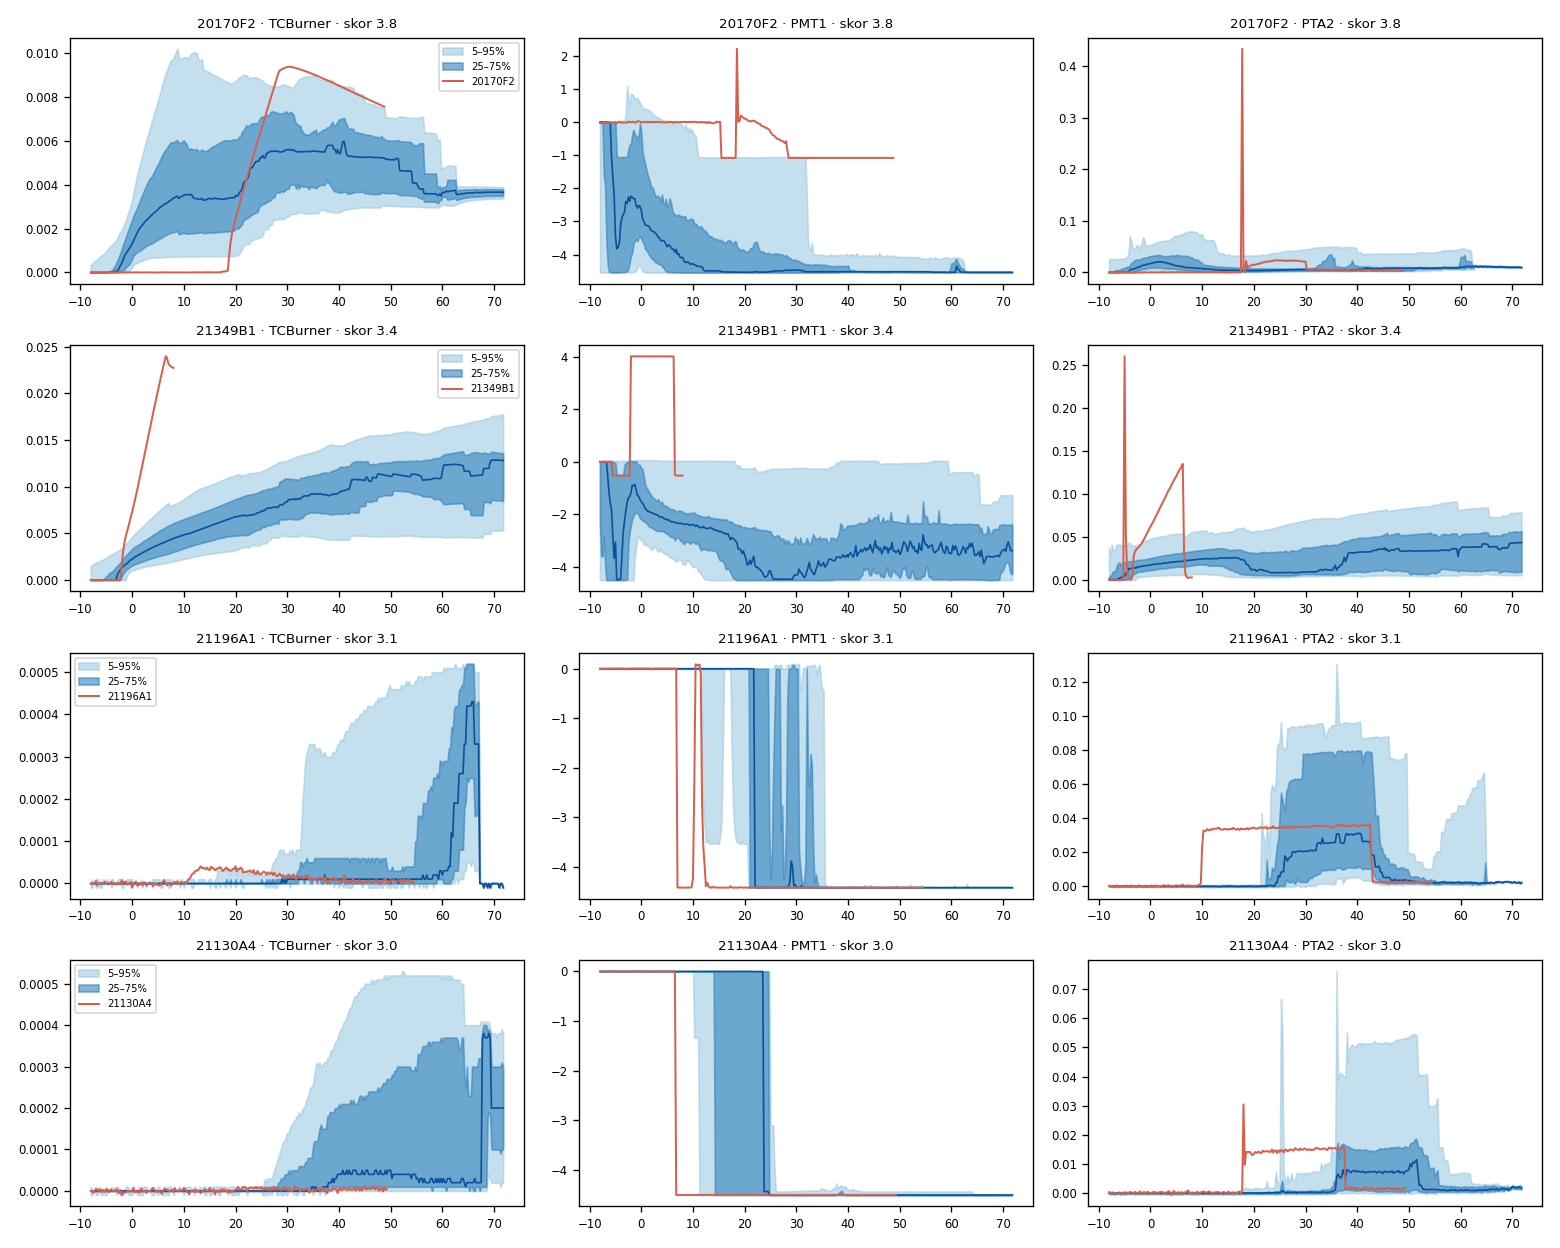
\includegraphics[width=\linewidth]{top_anomalies.png}
\caption{Uji dengan skor anomali tertinggi di atas koridor kelompoknya
(\texttt{analysis/telemetry/corridor/top\_anomalies.png}).}
\label{fig:koridor}
\end{figure}

% =====================================================================
\chapter{Analisis video BASS}\label{bab:video}

\section{Masalah dan metode}

Tabel uji BASS dan BASS-II memuat 251 baris tanpa satu pun hasil. Skrip
\berkas{scripts/video_analyze.py} mengukur nyala dari video: durasi nyala tampak per episode,
waktu mulai dan padam, luas tampak (piksel), cara berakhir (bertahap atau mendadak), dan
geseran sentroid. Skrip \berkas{scripts/video_join.py} lalu memasangkan setiap episode ke baris
tabel uji lewat kode uji, sehingga durasi nyala berdampingan dengan material, \Od, dan setelan
aliran.

Yang \emph{tidak} diklaim: satuan fisis mutlak (tanpa penanda skala, luas tetap dalam piksel),
laju rambat (pada sampel batang api memang menetap di ujung), dan anggapan bahwa setiap wilayah
terang adalah api.

\section{Empat kegagalan yang ditemukan lewat lembar bukti}

Keempatnya ditemukan dengan melihat lembar bukti, bukan dari angka. Angkanya terlihat wajar
di keempat kasus, dan karena itulah lembar bukti wajib diperiksa.

\begin{enumerate}
\item Berkas \texttt{\_2ND\_VIEW} ternyata kamera luar yang menyorot kotak sarung tangan beserta
      astronot. Pantulannya terbaca sebagai api selama 425 sampai 509 detik. Diperbaiki dengan
      gerbang adegan: median frame nyala sejati 0, interior saluran bersorot 30, kamera luar
      84 sampai 93; ambangnya 8.
\item Tepi sampel yang tersorot lampu terbaca sebagai api memanjang. Disaring lewat rasio sisi.
\item Potret layar LCD kamera Nikon terselip di sebagian video. Disaring lewat rasio isi.
\item Dua episode tergabung jadi satu: video P1 memuat dua segmen yang dipisahkan jeda gelap
      44 detik. Kini dipisah per episode.
\end{enumerate}

\section{Hasil}

Pilot (\berkas{analysis/video_pilot/}, 30 video) menghasilkan 37 episode; ke-37 cocok ke baris
tabel NASA dan tidak satu pun punya kolom hasil di tabel. Jalan penuh
(\berkas{analysis/video_full/}) mencakup 96 video BASS-II dengan 139 episode pembakaran. Median
durasi nyala per material ada di Tabel~\ref{tab:uq-video} (Bab~\ref{bab:statistik}).

\catatan{Ketelitian belum dapat ditetapkan}{Angka ketelitian ``$\pm$12~persen'' sempat ditulis lalu dicabut. Ternyata sebagian besar pasangan
video yang dikira rekaman ulang uji yang sama sebenarnya kejadian berbeda (dua penyalaan, dua
potongan berurutan, klip cuplikan, rekaman layar). Hanya uji T16 yang benar-benar terekam ulang
(selisih 6 dan 17~persen pada dua episodenya). Satu uji terlalu sedikit untuk mengklaim ketelitian
metode. Durasi dari video sah sebagai ukuran kasar dengan tingkat \tier{derived\_auto}.}

Dugaan awal bahwa jumlah episode sama dengan jumlah setelan aliran di kolom \texttt{Air display}
juga tidak terbukti (cocok 5 dari 16). Alasannya fisis: mengubah aliran di tengah pembakaran
tidak memadamkan api, dan penyalaan ulang pada setelan yang sama menghasilkan beberapa episode.

\section{Verifikasi manusia}

Skrip \berkas{scripts/proof_review.py} membuat \berkas{analysis/video_full/review.html}, halaman
untuk memeriksa 90 lembar bukti satu per satu dan memberi putusan OK, Salah, atau Ragu. Video
yang paling mungkin salah tampil paling atas. Hasil putusan diekspor ke \berkas{review.csv} lalu
diterapkan dengan \texttt{proof\_review.py --apply}, yang menulis
\berkas{measurements_verified.csv}. Hanya episode dari video berputusan OK yang boleh dipakai
sebagai agregat di dashboard. Pemeriksaan ini belum dilakukan, sehingga semua angka video masih
\tier{derived\_auto}. Gambar~\ref{fig:video} adalah contoh lembar bukti.

\begin{figure}[ht]
\centering
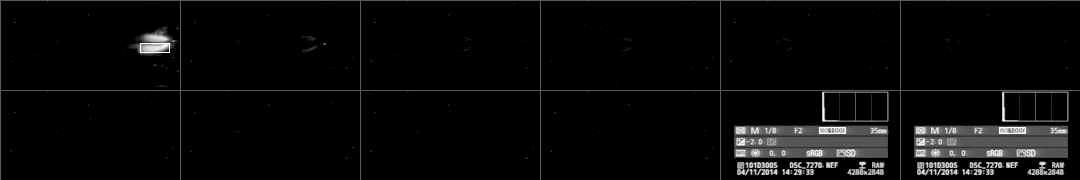
\includegraphics[width=0.75\linewidth]{video_bukti_T5.png}
\caption{Contoh lembar bukti video BASS-II uji T5: montase frame dengan kotak deteksi nyala.}
\label{fig:video}
\end{figure}

% =====================================================================
\chapter{Laju rambat api Saffire}\label{bab:saffire}

\section{Data}

Saffire-I (PSI-98) dan Saffire-III (PSI-100) merekam kebakaran sampel kain besar dengan dua
kamera. NASA sudah memetakan citranya (\asing{Mapped}: distorsi lensa diluruskan). Kamera
bergantian merekam dua jenis frame: frame gelap yang hanya memperlihatkan nyala, dan frame
terang yang menyinari sampel dari belakang sehingga kain utuh tampak hijau terang dan bagian
yang terbakar gelap. Total sekitar 112 ribu frame. Untuk Saffire-III, zip bagian 1 sampai 4
(sekitar 750~MB) diunduh karena bagian 4 saja tidak memuat nyala.

\section{Metode}

Skrip \berkas{scripts/saffire_spread.py} mengukur dua front secara terpisah:
\begin{itemize}
\item \textbf{Ujung api} dari frame gelap: profil kanal merah per kolom. Frame dianggap berisi
      nyala jika dominan merah dan median kanal hijaunya di bawah 8.
\item \textbf{Front hangus} dari frame terang: tempat kanal hijau jatuh per baris, diambil
      mediannya. Front hanya diukur selama paling sedikit 2~persen pita sampel masih terang,
      dengan ambang mutlak. Tanpa syarat ini, detektor sempat menangkap tepi bingkai setelah
      kain habis terbakar.
\end{itemize}

\textbf{Skala} ditentukan dengan dua cara. Untuk Saffire-I ada citra kisi distorsi berpola papan
catur 30~mm; satu periode pola sama dengan 60~mm, dan periodenya dicari dari puncak spektrum
FFT. Skala ditolak jika arah $x$ dan $y$ berbeda lebih dari 5~persen. Cara autokorelasi sempat
dipakai dan gagal karena memilih kelipatan periode (6,58 lawan 3,47~px/mm). Saffire-III tidak
punya citra kisi, jadi skalanya diambil dari tinggi bidang sampel yang terang pada frame awal,
yaitu lebar sampel 406~mm. Cara kedua ini diuji silang pada Saffire-I dan memberi 40,4~cm
terhadap skala kisi (selisih 0,5~persen).

\textbf{Laju} dihitung dengan regresi Theil-Sen posisi terhadap waktu pada fase rambat tunak
(10 sampai 90~persen lintasan). Selang 95~persen berasal dari bootstrap blok waktu, karena
frame berurutan saling berkorelasi.

\textbf{Gerbang mutu} ditetapkan buta terhadap angka publikasi: hasil lolos jika residu RMS di
bawah 20~mm dan lebar selang 95~persen di bawah 20~persen laju. Hasil yang gagal tetap dilaporkan
dengan tanda, tidak dibuang.

\section{Hasil}

\begin{table}[ht]
\centering\small
\caption{Laju rambat Saffire (\texttt{analysis/saffire/spread\_rates.csv}). Publikasi: paper
``Flame spread: Effects of microgravity and scale'', hlm.~13.}
\label{tab:saffire}
\begin{tabular}{@{}l l r l r r l@{}}
\toprule
Kamera & Front & mm/s & CI95 & Publikasi & Selisih & Mutu\\
\midrule
Saffire-I, kamera 1 & ujung api & 1,815 & [1,794; 1,841] & 1,8 & +0,8\,\% & lolos\\
Saffire-I, kamera 1 & front hangus & 1,062 & [0,034; 1,784] & 1,8 & $-$41,0\,\% & gagal\\
Saffire-I, kamera 2 & ujung api & 1,924 & [1,896; 1,953] & 1,8 & +6,9\,\% & lolos\\
Saffire-I, kamera 2 & front hangus & 1,881 & [1,814; 1,941] & 1,8 & +4,5\,\% & lolos\\
Saffire-III, kamera 1 & ujung api & 2,255 & [2,242; 2,268] & 2,3 & $-$2,0\,\% & lolos\\
Saffire-III, kamera 1 & front hangus & 2,159 & [2,102; 2,226] & 2,3 & $-$6,1\,\% & lolos\\
Saffire-III, kamera 2 & ujung api & 2,421 & [2,382; 2,451] & 2,3 & +5,3\,\% & lolos\\
Saffire-III, kamera 2 & front hangus & 1,373 & [0,619; 2,000] & 2,3 & $-$40,3\,\% & gagal\\
\bottomrule
\end{tabular}
\end{table}

Keempat pengukuran ujung api berada dalam $-$2 sampai +7~persen dari angka publikasi
(1,8~mm/s untuk Saffire-I pada aliran 20~cm/s; 2,3~mm/s untuk Saffire-III pada 25~cm/s). Angka
publikasi itu tidak dipakai untuk memilih parameter apa pun; ia baru dibandingkan setelah hasil
keluar. Dua front hangus gagal gerbang mutu, dan gerbang itu menangkapnya tanpa melihat angka
publikasi. Gambar~\ref{fig:saffire} memperlihatkan lembar bukti salah satu kamera.

\begin{figure}[ht]
\centering
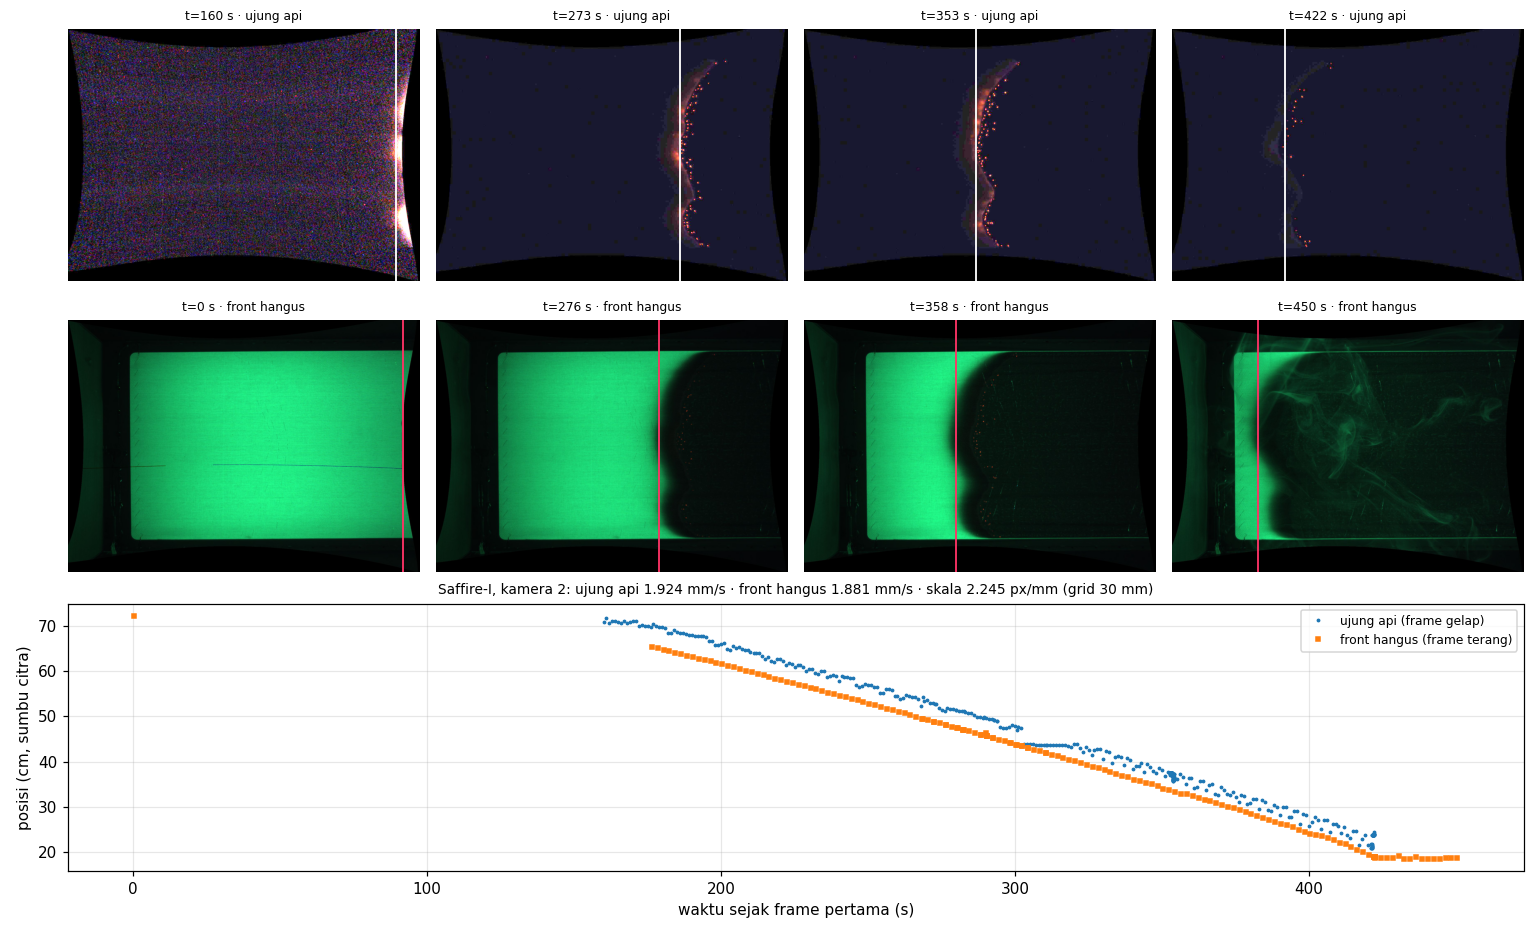
\includegraphics[width=\linewidth]{saffire1_C2.png}
\caption{Lembar bukti Saffire-I kamera 2. Baris atas: frame gelap dengan ujung api terdeteksi
(garis putih). Baris tengah: frame terang dengan front hangus (garis merah). Bawah: posisi
terhadap waktu; kedua front sejajar.}
\label{fig:saffire}
\end{figure}

\section{Temuan: dua sumber tidak sepakat}

Tabel uji NASA mencatat aliran Saffire-III sebesar 30~cm/s, sedangkan paper yang sama
(hlm.~6) mencatat 25~cm/s. Perbedaan ini ditangkap aturan R6 di otak dan ditampilkan sebagai
peringatan kritis. Kami tidak memutuskan mana yang benar; keduanya ditampilkan berdampingan
dengan sumbernya. Semua angka Saffire masuk otak sebagai \tier{derived\_auto} dengan tanda
\texttt{belum\_diverifikasi\_manusia}, dan angka publikasinya sebagai \tier{paper\_claim}.

% =====================================================================
\chapter{Model pembelajaran mesin}\label{bab:ml}

\section{Mengapa validasi per hari}

Uji pada hari yang sama berbagi gas ruang, kalibrasi, dan kru, sehingga hasilnya mirip satu sama
lain. Validasi silang acak menaruh uji sehari di data latih dan data uji sekaligus, sehingga angka
validasinya terlalu optimistis. Semua model di workspace ini divalidasi dengan
\asing{GroupKFold} per hari uji. Angka itu menjawab pertanyaan yang sebenarnya: seberapa baik
model untuk hari uji yang belum pernah dilihat.

\section{Model awal}

Skrip \berkas{scripts/build_model.py} membuat model generasi pertama yang sederhana dan bisa
dijelaskan: regresi linear laju bakar FLEX dan regresi logistik untuk peluang padam FLEX, peluang
menyala CFI-G, dan peluang padam sendiri CFI-G. Hasilnya ada di \berkas{kb/gold/model_params.json}
dan \berkas{kb/gold/model_report.md}, lalu dipakai simulator \berkas{app/freefall_lab.html}.
Model ini divalidasi secara acak, jadi angkanya tidak sebanding dengan angka per hari di bawah.

\section{Model tabular lanjutan}

Skrip \berkas{scripts/ml_tabular.py} membandingkan delapan jenis model pada empat target. Fitur
hanya kondisi yang direncanakan; kolom hasil sengaja tidak dipakai. Laporan lengkapnya di
\berkas{analysis/ml/tabular_report.md}.

\begin{table}[ht]
\centering\small
\caption{Model terbaik per target (validasi per hari). Kolom ``acak'' memperlihatkan seberapa
optimistis validasi acak.}
\begin{tabularx}{\linewidth}{@{}X l r r r@{}}
\toprule
Target & Model terbaik & Per hari & Model lama & Acak (lama)\\
\midrule
CFI-G: P(menyala), $n=325$, 23 hari & proses Gaussian & AUC 0,858 & AUC 0,649 & 0,787\\
CFI-G: P(padam sendiri $\mid$ menyala), $n=263$ & gradient boosting & AUC 0,889 & AUC 0,690 & 0,753\\
FLEX: P(padam sebelum droplet habis), $n=206$ & logistik (lama) & AUC 0,820 & AUC 0,820 & 0,810\\
FLEX: laju bakar $K$, $n=257$, 80 hari & ridge (lama) & RMSE 0,089 & RMSE 0,089 & \\
\bottomrule
\end{tabularx}
\end{table}

Pelajarannya: CFI-G butuh model nonlinear, dan validasi acak di sana jauh terlalu optimistis.
FLEX tidak; model linear lama tetap terbaik. Jaringan saraf MLP tidak unggul pada tabel sekecil
ini dan paling buruk untuk $K$ (R\textsuperscript{2} per hari $-$0,013). Pelatihan dijalankan di
klaster quasi09; model \asing{stacking} dihentikan karena membebani klaster bersama.

\section{Deep learning pada telemetri}

Skrip \berkas{scripts/ml_telemetry_prep.py} mengubah setiap rekaman menjadi tensor berukuran
tetap: 18 kanal yang sama di ketiga investigasi ACME, dicuplik ulang ke 4~Hz selama 128~detik,
dikurangi nilai dasar per kanal (\berkas{analysis/ml/telemetry_tensors.npz}). Skrip
\berkas{scripts/ml_telemetry_dl.py} melatih ResNet 1-D multi-tugas (menyala, padam sendiri,
waktu bakar) dengan label NASA PSI-159, sebagai ansambel 5 lipatan kali 5 benih di GPU RTX~3080.

\begin{table}[ht]
\centering\small
\caption{Perbandingan pada 320 uji PSI-159, validasi per hari
(\texttt{analysis/ml/telemetry\_dl\_results\_gpu\_w32.json}).}
\begin{tabular}{@{}l r r r r@{}}
\toprule
Metode & Menyala AUC & Menyala akurasi & Padam sendiri AUC & MAE waktu bakar\\
\midrule
Aturan termokopel 0,0006~V & 0,971 & 0,938 & & \\
Hanya median & & & & 35,1~s\\
Fitur buatan tangan + GB & 0,990 & 0,956 & 0,940 & 9,8~s\\
CNN dari nol & 0,988 & 0,969 & 0,983 & 12,7~s\\
CNN dengan pra-latih & 0,992 & 0,953 & 0,976 & 14,0~s\\
\bottomrule
\end{tabular}
\end{table}

CNN paling unggul untuk padam sendiri (AUC 0,983 lawan 0,940), sedangkan fitur buatan tangan
paling baik untuk waktu bakar. Pra-latih swa-awasan (merekonstruksi bentang sinyal yang
ditutupi, pada sekitar 600 rekaman PSI-10 dan PSI-23 tanpa label) \emph{tidak} membantu dan
dilaporkan apa adanya. Analisis oklusi menunjukkan kanal paling berpengaruh adalah termokopel
burner dan tekanan ruang PTA2/PTA3, sesuai fisikanya. Tiga varian disimpan: CPU, GPU lebar 32,
dan GPU lebar 64. Yang masuk otak adalah GPU lebar 32 (kartu \texttt{cnn\_telemetry\_w32}).

Ansambel lalu memprediksi PSI-10 dan PSI-23, yang tidak punya label NASA. Ini ekstrapolasi ke
investigasi lain. Kesepakatannya dengan aturan termokopel 99,7~persen di PSI-10 dan 97,2~persen
di PSI-23; uji dengan simpangan antar-model di atas 0,2 ditandai ragu (4 dan 15 uji).

Model gradient boosting kecil atas fitur telemetri (\berkas{scripts/ml_labels.py}) dilatih ulang
otomatis setiap kali ada label manusia baru (Bab~\ref{bab:belajar}). Saat ini, tanpa label manusia,
AUC-nya 0,992 terhadap label NASA.

\section{Peta batas dan rekomendasi uji berikutnya}

Skrip \berkas{scripts/ml_boundary.py} mempelajari batas menyala atau tidak (CFI-G) dan batas padam
(FLEX) dengan klasifikasi proses Gaussian, lalu memakai fungsi-U $U(x) = |\mu(x)|/\sigma(x)$
(Schmidt, bab 9.4) untuk menunjuk kondisi yang paling mungkin salah diklasifikasi. Kondisi dengan
$U$ terkecil adalah uji berikutnya yang paling informatif.

Kandidat uji diambil dari kondisi uji nyata yang digeser sedikit (sekitar 5~persen rentang).
Sampel acak di seluruh ruang kondisi sempat dicoba dan gagal: jauh dari data, proses Gaussian
kembali ke prior sehingga $U \approx 0$ secara trivial, dan kombinasi yang tidak pernah diuji ikut
muncul. Validasi per hari: CFI-G AUC 0,845 (logistik 0,658); FLEX AUC 0,821 (logistik 0,789).
Keluaran: \berkas{analysis/ml/boundary/boundary.json} dan peta di Gambar~\ref{fig:batas}.

\begin{figure}[ht]
\centering
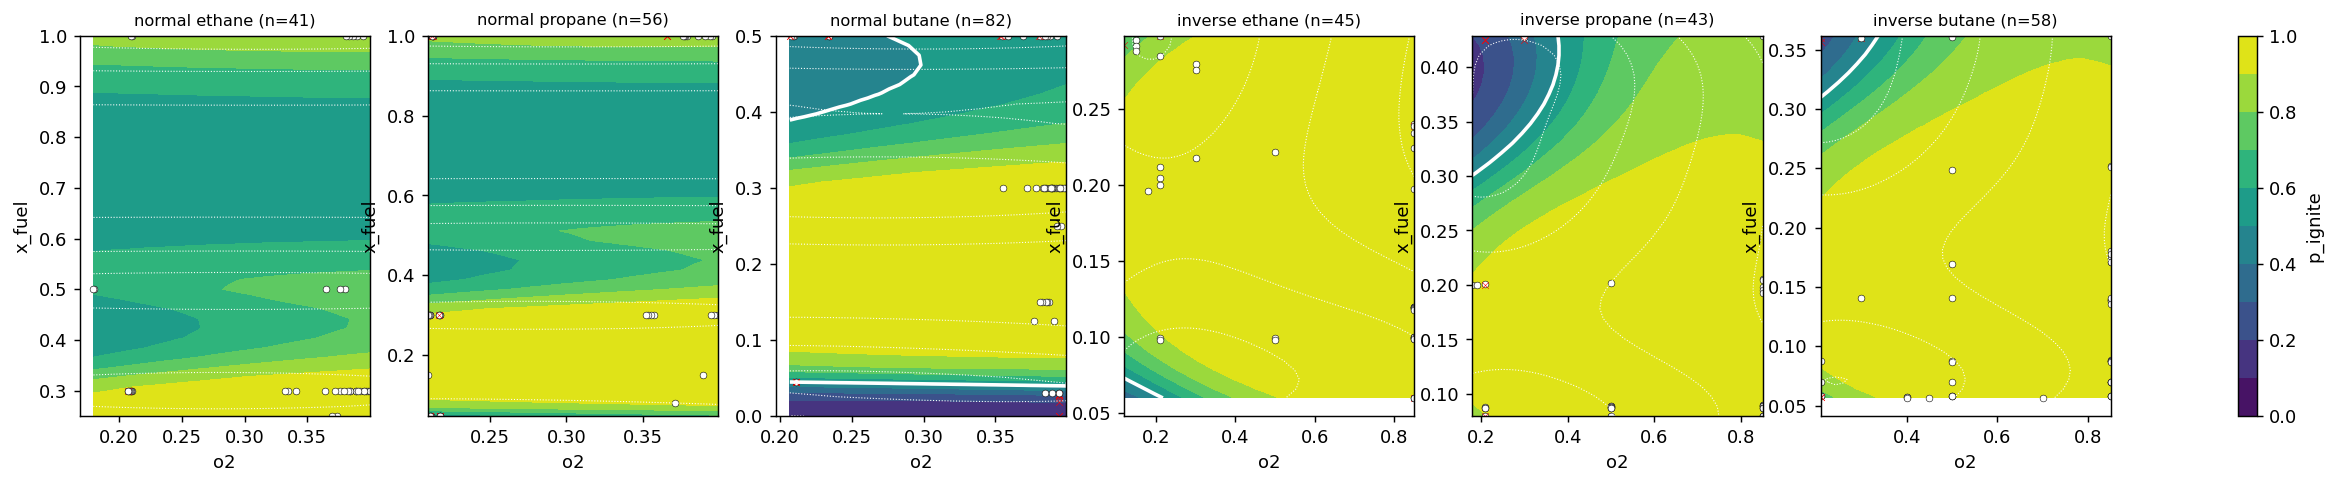
\includegraphics[width=\linewidth]{cfig_ignition_map.png}
\caption{Peluang menyala CFI-G per konfigurasi dan bahan bakar, terhadap \Od{} dan fraksi bahan
bakar. Garis putih tebal adalah batas $P=0{,}5$; titik adalah uji nyata.}
\label{fig:batas}
\end{figure}

\section{Rumus laju bakar droplet}

Skrip \berkas{scripts/symreg_flex.py} mencari rumus jarang untuk laju bakar FLEX dari pustaka suku
yang diturunkan dari teori hukum $d^2$. Hasil terpilih (aturan 1-SE, RMSE per hari 0,0899):
\[
K \approx 0{,}111 + 1{,}8\,X_{\mathrm{O_2}} + 0{,}611\,X_{\mathrm{He}} \quad (\text{mm}^2/\text{s}).
\]
Model linear lima fitur memberi RMSE 0,0832 dan model terbaik dari pencarian menyeluruh 0,0823,
jadi rumus dua suku ini hampir sama baiknya dengan jauh lebih sedikit parameter. Percobaan pertama
dengan STLS (gaya SINDy) gagal: semua bentuk \Od{} dipertahankan sekaligus dengan koefisien sampai
$10^6$ yang saling meniadakan karena suku-sukunya hampir kolinear. Solusinya membatasi satu bentuk
\Od{} per model. Rumus ini empiris dan hanya berlaku di rentang kondisi FLEX
(\berkas{analysis/ml/symreg_flex.md}).

\section{Waktu bakar sebagai rentang}

Waktu bakar CFI-G bersifat bimodal: nyala yang padam sendiri berumur pendek, sedangkan yang
dihentikan operator berumur panjang. Skrip \berkas{scripts/ml_quantile.py} memprediksi persentil
10, 50, dan 90 dengan gradient boosting kuantil. Sebelum kalibrasi, hanya 62,7~persen uji jatuh di
rentang P10 sampai P90 (target 80~persen). Setelah kalibrasi konformal per hari, cakupannya
85,9~persen dengan lebar median 74,5~detik (\berkas{analysis/ml/quantile_burn.json}).

% =====================================================================
\chapter{Ketidakpastian statistik}\label{bab:statistik}

Skrip \berkas{scripts/stats_uq.py} menghitung selang 95~persen dengan \textbf{bootstrap cluster
per hari uji} (4000 ulangan): yang diambil ulang adalah hari, bukan uji satu per satu. Bootstrap
per uji (kolom ``naif'') ditampilkan sebagai pembanding untuk memperlihatkan seberapa sempit
selang jika korelasi antar-uji sehari diabaikan. Laporan lengkap ada di
\berkas{analysis/stats/uq_report.md}.

\begin{table}[ht]
\centering\small
\caption{Peluang menyala CFI-G per kelompok.}
\begin{tabular}{@{}l r r r l l@{}}
\toprule
Kelompok & $n$ & Hari & Laju & CI95 cluster & CI95 naif\\
\midrule
normal etana & 41 & 3 & 0,976 & [0,923; 1,000] & [0,927; 1,000]\\
normal propana & 56 & 3 & 0,714 & [0,625; 1,000] & [0,589; 0,821]\\
normal butana & 82 & 5 & 0,634 & [0,398; 0,929] & [0,524; 0,732]\\
inverse etana & 45 & 4 & 0,911 & [0,821; 0,979] & [0,822; 0,978]\\
inverse propana & 43 & 4 & 0,861 & [0,536; 0,984] & [0,744; 0,954]\\
inverse butana & 58 & 4 & 0,914 & [0,827; 1,000] & [0,844; 0,983]\\
\bottomrule
\end{tabular}
\end{table}

Selisih laju menyala inverse dikurangi normal adalah +0,160 dengan $p$ permutasi 0,0012, tetapi
selang bootstrap cluster-nya $[-0{,}021;\ +0{,}321]$ masih mencakup nol. Uji permutasi biasa
menganggap setiap uji independen, padahal konfigurasi biasanya tetap sepanjang hari. Kesimpulan
yang jujur: inverse \emph{cenderung} lebih mudah menyala, tetapi belum terbukti.

Untuk FLEX, laju bakar heptana lebih tinggi dari metanol sebesar +0,0729~mm\textsuperscript{2}/s
(CI95 cluster $[+0{,}0199;\ +0{,}1263]$), dan heptana dengan helium lebih tinggi +0,1315
(CI95 $[+0{,}0443;\ +0{,}2313]$). Helium biasanya diuji bersama \Od{} dan tekanan yang berbeda,
jadi angka ini asosiasi, bukan efek sebab-akibat murni.

\begin{table}[ht]
\centering\small
\caption{Durasi nyala per episode dari video BASS-II, belum diverifikasi manusia.}
\label{tab:uq-video}
\begin{tabular}{@{}l r r r l@{}}
\toprule
Material & Episode & Uji & Median (s) & CI95 cluster per uji\\
\midrule
batang bening 1/4'' & 18 & 9 & 39,5 & [22,2; 90,2]\\
SIBAL 2~cm & 17 & 12 & 8,0 & [6,0; 15,8]\\
batang hitam 1/4'' & 16 & 6 & 70,0 & [9,0; 159,0]\\
batang bening 3/8'' & 9 & 2 & 66,5 & [52,5; 103,8]\\
SIBAL 1~cm & 9 & 7 & 7,5 & [5,5; 9,0]\\
potongan bola 4~cm & 8 & 2 & 51,2 & [26,5; 65,0]\\
batang PMMA bening 1/2'' & 6 & 3 & 134,5 & [57,0; 212,0]\\
\bottomrule
\end{tabular}
\end{table}

Durasi bakar dari telemetri (median, CI95 cluster) adalah 44,6~s [37,9; 53,5] untuk PSI-10,
26,3~s [23,6; 30,3] untuk PSI-23, dan 51,7~s [44,3; 59,9] untuk PSI-159. Angka ini cenderung
berlebih karena jeda termal termokopel.

% =====================================================================
\chapter{Otak: graf pengetahuan bertingkat kebenaran}\label{bab:otak}

\section{Isi}

Skrip \berkas{scripts/build_brain.py} menyatukan semua hasil di atas ke
\berkas{kb/gold/brain.sqlite}. Skrip ini tidak menghitung ulang analisis apa pun; ia hanya
membaca keluaran yang sudah ada. Otak disimpan terpisah dari \berkas{freefall.sqlite} supaya
\texttt{build\_kb.py} tidak menghapusnya.

\begin{table}[ht]
\centering\small
\caption{Tabel di \texttt{brain.sqlite}.}
\begin{tabularx}{\linewidth}{@{}l r X@{}}
\toprule
Tabel & Baris & Isi\\
\midrule
\texttt{entity} & \bEntity & 24 investigasi, 1928 uji, 695 paper\\
\texttt{artifact} & \bArtifact & 943 rekaman telemetri, 83 video, 10 deret citra\\
\texttt{measurement} & \bMeas & Setiap angka: besaran, nilai, satuan, selang, tingkat kebenaran, metode, berkas dan lokasi sumber, tanda, pemverifikasi\\
\texttt{link} & \bLink & Tautan antar-entitas: hari yang sama, seri sebelum dan sesudah, bagian dari investigasi, punya artefak, diringkas oleh baris kampanye\\
\texttt{rule} & \bRule & Aturan deduktif, disimpan sebagai data\\
\texttt{rule\_hit} & \bRuleHit & Setiap kali aturan mengenai satu entitas atau angka\\
\texttt{model\_card} & \bCard & Kartu model: target, metode, metrik, rentang berlaku, catatan\\
\bottomrule
\end{tabularx}
\end{table}

Pembangunan otak bersifat atomik: data ditulis dulu ke berkas sementara lalu ditukar dengan
\texttt{os.replace}, sehingga server yang sedang berjalan tidak pernah membaca basis data
setengah jadi. Pada Windows, berkas yang sedang dibuka server tidak bisa ditukar dari proses
lain. Karena itu pembangunan ulang saat server hidup harus dipicu lewat server
(\texttt{POST /rebuild}), yang menutup koneksinya sebentar selama penukaran.

\section{Aturan}

\begin{table}[ht]
\centering\small
\caption{Enam aturan deduktif dan jumlah entitas yang dikenainya saat ini.}
\begin{tabularx}{\linewidth}{@{}l X X r@{}}
\toprule
Aturan & Kondisi & Akibat & Kena\\
\midrule
R1 sinyal lemah & telemetri menyala dan kenaikan termokopel $<$ 0,002~V & tanda \texttt{sinyal\_lemah}, tetap ditampilkan & 118\\
R2 percobaan ulang & uji hanya ada di telemetri, tidak menyala, dan uji berikutnya di seri yang sama ada & tanda \texttt{kemungkinan\_percobaan\_ulang} & 9\\
R3 tanpa konsumsi \Od & uji hanya di telemetri dinyatakan menyala, tetapi \Od{} akhir uji sebelumnya sama persis dengan \Od{} awal uji sesudahnya & tanda \texttt{kemungkinan\_positif\_palsu} & 1\\
R4 kanal aliran inverse & sinyal aliran bahan bakar pada konfigurasi inverse & tanda \texttt{kanal\_tak\_informatif} & 248\\
R5 catatan operator & uji punya catatan operator NASA & ditautkan sebagai bukti untuk ``kenapa'' & 868\\
R6 beda sumber & nilai yang sama dari tabel NASA dan paper berbeda lebih dari 10~persen & tanda \texttt{sumber\_bertentangan}, peringatan kritis & 1\\
\bottomrule
\end{tabularx}
\end{table}

Setiap aturan menyimpan alasan dan asal temuannya, misalnya R3 berasal dari analisis uji 21106 G8.
Dengan begitu tabel aturan sekaligus menjadi dokumentasi yang selalu mutakhir.

\section{Peringatan, penjelasan, dan relevansi}

Dari aturan dan perbandingan sumber, otak memunculkan peringatan bertingkat: saat ini 20
\textbf{kritis} (dua sumber bertentangan, misalnya tabel NASA ``tidak menyala'' tetapi telemetri
``menyala''), 61 \textbf{perhatian} (kemungkinan positif palsu, sinyal lemah yang bertentangan),
dan 119 \textbf{info}. Peringatan yang sudah diputus manusia tidak dimunculkan lagi.

Fungsi \texttt{explain} di \berkas{scripts/brain.py} menyusun hipotesis ``kenapa'' untuk satu uji,
berperingkat menurut bobot, masing-masing dengan bukti dan sumbernya: aturan yang kena, catatan
operator, konteks seri, tetangga dalam ruang kondisi, dan putusan manusia jika ada (bobot
tertinggi). Fungsi \texttt{relevance} mengurutkan entitas lain menurut derajat keterkaitan dengan
fokus (seri, hari, kondisi serupa, paper yang menyebutnya). Fungsi \texttt{provenance} menelusuri
rantai asal-usul satu angka sampai ke berkas dan barisnya.

% =====================================================================
\chapter{Siklus belajar}\label{bab:belajar}

\section{Log anotasi}

Putusan manusia ditulis ke \berkas{kb/gold/annotations.jsonl} dan tidak pernah diubah atau
dihapus (\asing{event sourcing}). Otak selalu dibangun ulang dari data mentah ditambah log ini,
sehingga setiap keputusan bisa ditelusuri dan diputar ulang. Arti putusan:

\begin{itemize}
\item \textbf{ok}: angka naik ke tingkat \tier{human\_verified};
\item \textbf{salah}: angka diberi tanda \texttt{ditolak\_manusia} dan keluar dari agregat serta peringatan;
\item \textbf{ragu}: tanda \texttt{diragukan\_manusia}.
\end{itemize}

Untuk besaran ``menyala'', manusia boleh memberi nilainya sendiri (ya atau tidak). Jika nilai itu
diberikan, putusan ok atau salah dihitung otomatis dengan membandingkannya dengan nilai turunan.
Saat dokumen ini ditulis, log anotasi asli masih kosong.

\section{Pipeline bergaya make}

Skrip \berkas{scripts/learn.py} menjalankan langkah-langkah berikut. Setiap langkah dijalankan
ulang hanya jika sidik jari masukan \emph{atau} keluarannya berubah (disimpan di
\berkas{kb/gold/pipeline_state.json}). Sidik jari keluaran ditambahkan setelah ketahuan bahwa
keluaran yang diubah tangan sempat dianggap masih segar.

\begin{enumerate}
\item \texttt{proof\_apply}: putusan video ke \berkas{measurements_verified.csv};
\item \texttt{ml\_labels}: latih ulang model menyala dari telemetri dengan label NASA ditambah label manusia;
\item \texttt{stats\_uq}: hitung ulang selang ketidakpastian;
\item \texttt{corridor}, \texttt{boundary}, \texttt{symreg}, \texttt{quantile}, \texttt{saffire}: hanya dengan \texttt{--full}, karena lambat;
\item \texttt{build\_brain}: bangun ulang otak;
\item riwayat: catat ringkasan ke \berkas{kb/gold/model_history.jsonl}.
\end{enumerate}

Jalan penuh terakhir (11 November 2026) selesai dalam 572 detik; langkah terlama adalah Saffire
(310 detik) dan koridor (173 detik).

\section{Antrean verifikasi}

Antrean mengurutkan angka yang paling layak diperiksa manusia menurut ketidakpastian kali dampak.
Contoh teratasnya adalah uji yang menurut tabel NASA menyala tetapi menurut telemetri tidak. Saat
ini antrean berisi 131 butir.

% =====================================================================
\chapter{Dashboard}\label{bab:dashboard}

\section{Server}

\berkas{scripts/brain.py serve --port 8765} menjalankan server HTTP yang menyajikan dashboard di
\url{http://127.0.0.1:8765/app/} dan API JSON. Titik GET: \texttt{tests}, \texttt{alerts},
\texttt{whatif/cfig}, \texttt{whatif/flex}, \texttt{entity}, \texttt{explain}, \texttt{relevance},
\texttt{provenance}, \texttt{coverage}, \texttt{search}, \texttt{notes}, \texttt{events},
\texttt{queue}, \texttt{history}, \texttt{pipeline}, \texttt{model\_cards},
\texttt{assistant\_status}. Titik POST: \texttt{note}, \texttt{annotate}, \texttt{rebuild},
\texttt{ask}, \texttt{feedback}. Setiap utas punya koneksi SQLite sendiri, dan permintaan
ditahan sebentar selama otak ditukar. Uji membuktikan 146 permintaan selama penukaran berjalan
tanpa satu galat pun.

\section{Sistem saraf}

\berkas{app/nerve/nerve.js} menyimpan \emph{satu} keadaan bersama: fokus, pilihan
(\asing{brushing}), filter, setelan what-if, relevansi terhadap fokus, peringatan, jejak, catatan,
percakapan asisten, antrean, dan status belajar. Setiap perubahan lewat satu pintu,
\texttt{dispatch(aksi, argumen, pelaku)}, yang dipakai manusia maupun asisten. Akibatnya setiap
panel selalu sepakat, setiap langkah bisa dibatalkan (\asing{undo}), keadaan bisa dibagikan
sebagai tautan, dan jejak mencatat siapa melakukan apa. Respons yang datang terlambat untuk fokus
lama dibuang. Dashboard menanyakan peristiwa server secara berkala, sehingga hasil siklus belajar
muncul tanpa memuat ulang halaman.

\section{Tampilan}

Desain visual (tahap F) dipasang di atas kerangka dan saraf itu tanpa mengubah kabelnya.
Gambar~\ref{fig:dash} memperlihatkan dashboard dengan fokus pada uji 21106 G8.

\begin{figure}[ht]
\centering
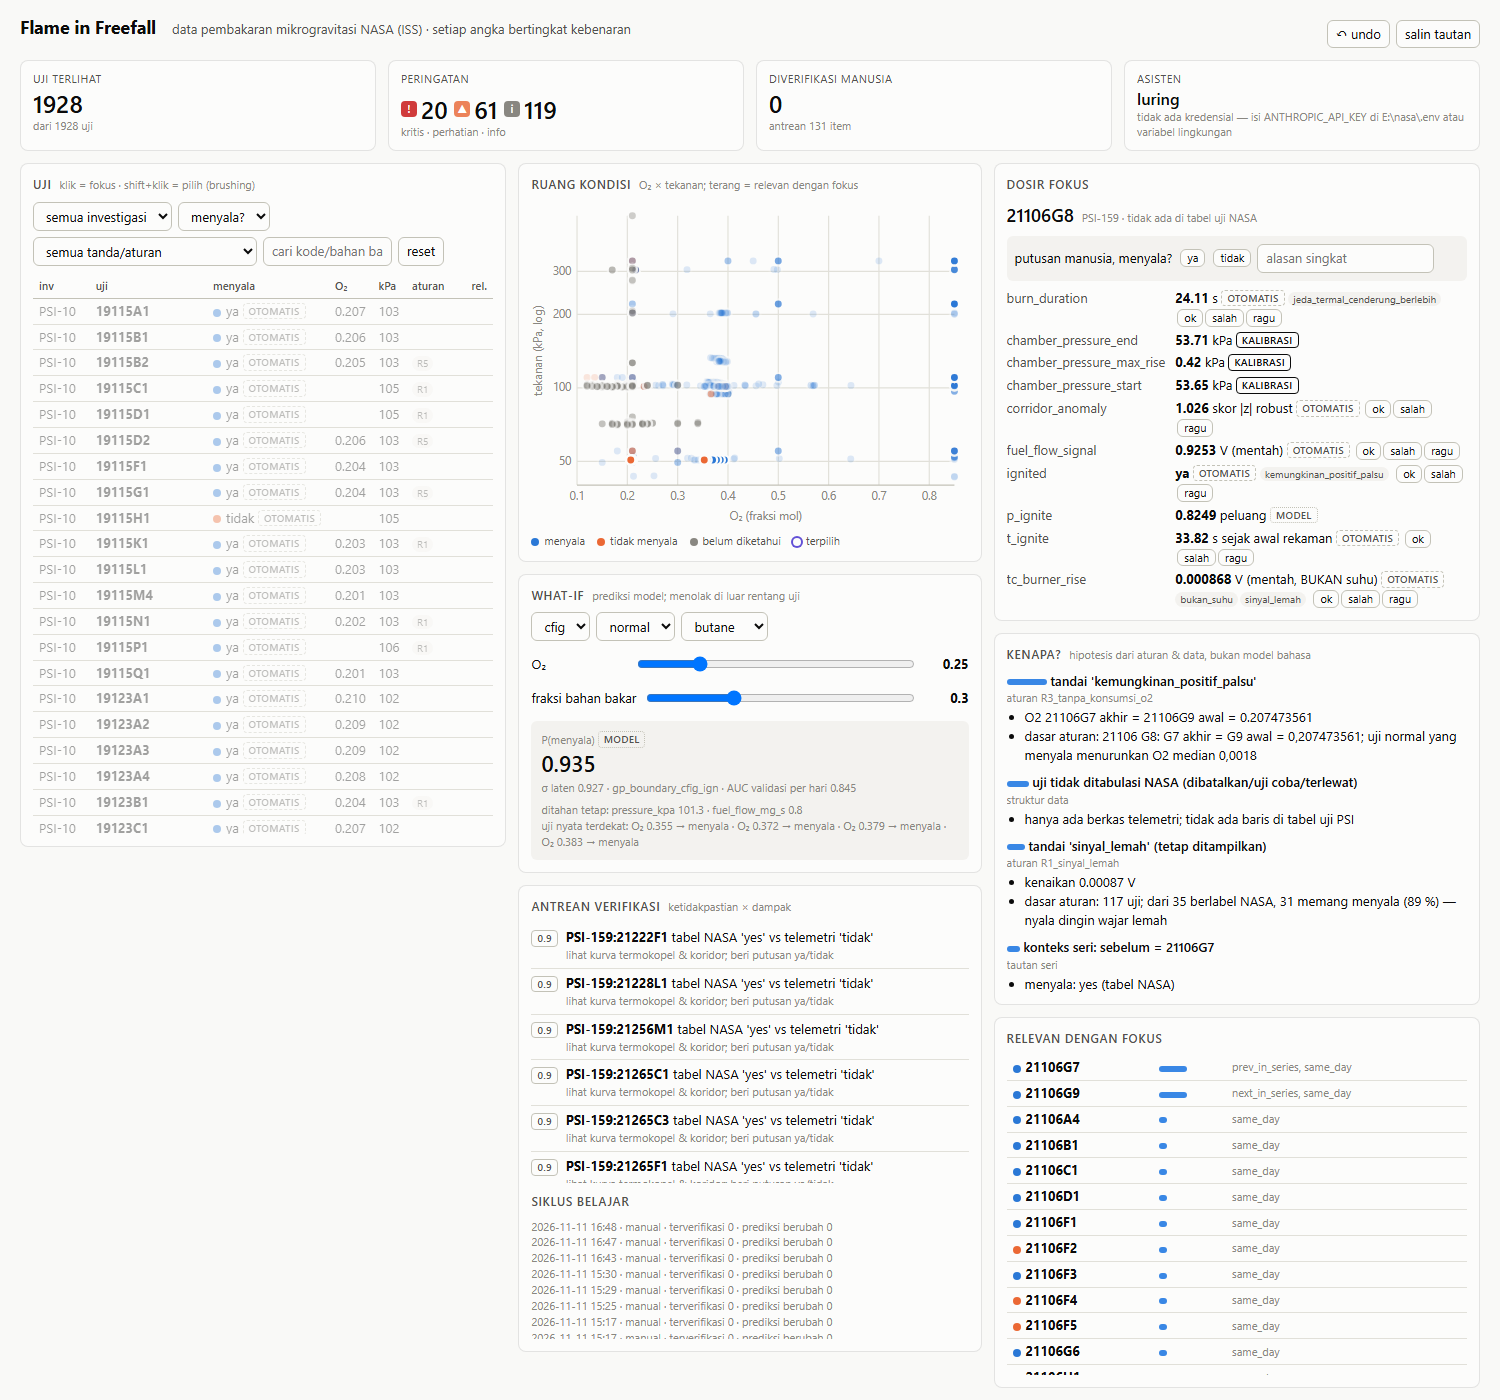
\includegraphics[width=\linewidth]{dashboard_terang.png}
\caption{Dashboard dalam tema terang, fokus pada uji 21106 G8. Baris atas: ubin ikhtisar.
Kolom kiri: daftar uji. Tengah: ruang kondisi, what-if, antrean verifikasi. Kanan: dosir fokus,
hipotesis ``kenapa'', dan entitas relevan.}
\label{fig:dash}
\end{figure}

Keputusan desainnya:
\begin{itemize}
\item \textbf{Ikhtisar dulu, rincian kemudian.} Empat ubin angka di atas (uji terlihat, peringatan
      per tingkat, jumlah terverifikasi manusia beserta panjang antrean, mode asisten).
\item \textbf{Warna mengikuti makna.} Menyala berwarna biru (\textcolor{biru}{\#2a78d6}), tidak
      menyala oranye (\textcolor{oranye}{\#eb6834}), belum diketahui abu-abu. Pasangan ini
      divalidasi dengan skrip validator palet untuk pembaca buta warna, pada tema terang dan gelap.
\item \textbf{Status tidak pernah hanya warna.} Peringatan selalu memakai ikon dan label (kritis,
      perhatian, info).
\item \textbf{Tingkat kebenaran sebagai lencana teks}: NASA, KALIBRASI, OTOMATIS, MANUSIA, PAPER,
      MODEL. Teksnya yang membawa makna; gaya garis hanya penegas.
\item \textbf{Grafik dengan sumbu, kisi, legenda, dan keterangan saat kursor diarahkan.} Tekanan
      digambar pada skala log.
\item \textbf{Tema gelap} memakai nilai warna gelapnya sendiri, bukan pembalikan otomatis.
\end{itemize}

Dari dosir, manusia memberi putusan per angka (ok, salah, ragu) atau putusan menyala (ya, tidak)
beserta alasan singkat. Putusan itu masuk log anotasi dan memicu siklus belajar.

\section{Aplikasi lain}

\berkas{app/freefall_lab.html} adalah simulator generasi pertama yang dibuat
\texttt{build\_model.py} dari \berkas{scripts/lab_template.html}, dengan data tertanam di satu
berkas. \berkas{app/hardware_lab.html} adalah penampil 3D perangkat eksperimen dengan model
skematik sementara, memakai three.js di \berkas{app/vendor/}. Spesifikasi model 3D untuk pemodel
ada di \berkas{docs/blender_3d_spec.md}.

% =====================================================================
\chapter{Asisten}\label{bab:asisten}

\section{Prinsip}

Asisten di \berkas{scripts/assistant.py} menjawab \emph{lewat alat}, bukan dari ingatan model
bahasa. Ada 15 alat, antara lain mencari uji, membuka dosir, menjelaskan ``kenapa'', menelusuri
asal-usul, membaca peringatan, menjalankan what-if, merekomendasikan uji berikutnya, mencari paper,
membaca kartu model, statistik ketidakpastian, antrean verifikasi, dan menggerakkan dashboard.
Asisten sengaja tidak diberi alat anotasi, karena verifikasi adalah pekerjaan manusia.

Beberapa aturan ditegakkan oleh kode, bukan hanya oleh instruksi:
\begin{itemize}
\item \textbf{Grounding}: setiap angka di jawaban harus muncul di keluaran alat. Angka yang tidak
      ditemukan dilaporkan di dashboard sebagai ``angka tanpa sumber''.
\item \textbf{Sitasi} berbentuk \texttt{[[test:...]]} atau \texttt{[[paper:judul|hlm]]} diubah menjadi
      daftar terstruktur lengkap dengan tingkat kebenarannya.
\item \textbf{Aksi dashboard} dari asisten dijalankan lewat pintu \texttt{dispatch} yang sama
      dengan manusia, dan tercatat di jejak sebagai pelaku ``asisten''.
\end{itemize}

\section{Dua mesin}

\textbf{Mode luring} adalah perencana deterministik: pengklasifikasi niat berbasis pola memilih alat
dan menyusun jawaban dari keluarannya. Mode ini berjalan tanpa internet dan menjadi mode aktif.

\textbf{Mode Claude} memakai model Claude dengan pemanggilan alat. Jalurnya sudah dibangun dan diuji
dengan API tiruan (\berkas{scripts/test_claude_mode.py}, 23 pemeriksaan, tanpa biaya). Mode ini
belum dipakai karena membutuhkan kunci API berbayar terpisah; langganan Claude Pro tidak termasuk
akses API. Kunci, jika kelak ada, hanya disimpan di \berkas{.env} yang dikecualikan dari git, dan
pemuatnya hanya membaca baris \texttt{ANTHROPIC\_*} tanpa pernah mencetak nilainya. Jika kunci
tidak ada atau API gagal, asisten jatuh ke mode luring dengan catatan.

\section{Evaluasi}

\begin{table}[ht]
\centering\small
\caption{Hasil evaluasi asisten mode luring.}
\begin{tabularx}{\linewidth}{@{}l r X@{}}
\toprule
Set & Hasil & Catatan\\
\midrule
Dev (\berkas{eval/assistant_eval.jsonl}) & 28/28 & Dipakai untuk mengembangkan; bukan ukuran generalisasi.\\
Hold-out 1 & & Sudah terpakai untuk perbaikan, lalu dipindah ke dev. Arsipnya di \berkas{arsip/eval/}.\\
Hold-out 2 (\berkas{eval/assistant_eval_holdout2.jsonl}) & 11/12 (91,7\,\%) & Dibekukan dengan SHA-1 sebelum dijalankan. Hanya jalan pertama yang sah. Kegagalan k08 lalu diperbaiki, sehingga set ini juga sudah terpakai.\\
\bottomrule
\end{tabularx}
\end{table}

Setiap pertanyaan dinilai pada lima aspek: alat yang dipanggil, isi wajib, isi terlarang (pola
yang tidak boleh muncul), aksi dashboard, dan grounding. Angka generalisasi yang sah untuk mode
luring adalah 91,7~persen pada 12 pertanyaan; sampel sekecil ini belum cukup untuk klaim yang kuat.

% =====================================================================
\chapter{Pengujian perangkat lunak}\label{bab:uji}

\begin{table}[ht]
\centering\small
\caption{Uji perangkat lunak dan hasil jalan terakhir (11 November 2026).}
\begin{tabularx}{\linewidth}{@{}l X l@{}}
\toprule
Uji & Yang diperiksa & Hasil\\
\midrule
\berkas{app/nerve/nerve.test.mjs} & Sistem saraf tanpa server: aksi, undo, tautan, respons basi & lulus\\
\berkas{app/nerve/nerve.live.mjs} & Ujung ke ujung terhadap server sungguhan: peringatan, fokus, filter, brushing, what-if di dalam dan di luar rentang & lulus\\
\berkas{app/nerve/nerve.learn.live.mjs} & Anotasi lewat server, siklus belajar, permintaan selama penukaran otak & lulus\\
\berkas{scripts/test_learning.py} & Siklus belajar dengan log sementara, lalu otak dipulihkan dari log asli & lulus\\
\berkas{scripts/test_claude_mode.py} & Jalur Claude dengan API tiruan: bentuk permintaan, loop alat, galat & 23/23\\
\texttt{assistant.py eval} & Mutu jawaban asisten (Bab~\ref{bab:asisten}) & 28/28 dev\\
\berkas{scripts/workspace_inventory.py} & Tidak ada berkas tanpa dokumentasi & 0 tak terdokumentasi\\
\bottomrule
\end{tabularx}
\end{table}

Uji yang menulis anotasi selalu memakai berkas sementara lewat variabel lingkungan
\texttt{FREEFALL\_ANN}, \texttt{FREEFALL\_STATE}, \texttt{FREEFALL\_HISTORY}, dan
\texttt{FREEFALL\_CASES}, sehingga log asli tidak tercemar. Setelah uji live, otak dibangun ulang
dari log asli.

% =====================================================================
\chapter{Temuan dan keterbatasan}\label{bab:temuan}

\section{Temuan utama}

\begin{enumerate}
\item Detektor nyala berbasis termokopel cocok 93,8~persen dengan penilaian NASA, sedangkan arus
      ion, yang tampak masuk akal, gagal (45,6~persen) karena CFI-G adalah nyala dingin.
\item 288 uji PSI-23 dipulihkan dari 18 baris ringkasan, dan 20 uji yang tidak ada di tabel NASA
      teridentifikasi beserta dugaan penyebabnya.
\item Rumus tekanan di lembar kerja NASA salah skala; rumus yang dikoreksi memberi galat 2,2~kPa
      tanpa fitting.
\item Skor anomali koridor, yang dihitung tanpa melihat komentar operator, lebih tinggi pada uji
      yang dikomentari NASA ($p = 0{,}001$).
\item Laju rambat api Saffire yang diukur dari citra berada dalam $-$2 sampai +7~persen dari angka
      publikasi, dengan gerbang mutu yang buta terhadap angka itu.
\item Tabel NASA dan paper berbeda tentang aliran Saffire-III (30 lawan 25~cm/s).
\item Validasi acak terlalu optimistis untuk CFI-G (AUC 0,787 lawan 0,649 per hari untuk model
      lama). Model nonlinear menaikkan AUC per hari menjadi 0,858 untuk menyala dan 0,889 untuk
      padam sendiri.
\item Laju bakar droplet FLEX dapat diringkas dengan rumus dua suku yang hampir setara dengan model
      lima fitur.
\item Perbedaan peluang menyala inverse dan normal belum terbukti setelah korelasi per hari
      diperhitungkan, meskipun uji permutasi biasa memberi $p = 0{,}0012$.
\end{enumerate}

\section{Keterbatasan}

\begin{itemize}
\item Belum ada angka \tier{human\_verified}. Semua hasil video, Saffire, dan sebagian telemetri
      masih menunggu pemeriksaan lembar bukti oleh manusia.
\item Kanal termokopel tetap dalam volt; tidak ada kurva kalibrasi suhu.
\item Ketelitian durasi dari video belum terkuantifikasi.
\item Semua model empiris dan hanya berlaku di rentang kondisi yang pernah diuji. Simulator what-if
      menolak menjawab di luar rentang itu.
\item Prediksi CNN untuk PSI-10 dan PSI-23 adalah ekstrapolasi tanpa label NASA.
\item Hanya \doiPdf{} dari \nPapersDoi{} paper ber-DOI yang punya teks lengkap; sisanya abstrak.
\item Hold-out asisten masih kecil (12 pertanyaan), dan mode Claude belum dievaluasi dengan API
      sungguhan.
\item Semua data adalah mikrogravitasi; tidak ada variabel gravitasi di model mana pun.
\item Workspace belum berada di bawah git, sehingga kolom versi kode di otak berisi
      \texttt{tanpa-git}. Sidik jari sha256 di inventaris menggantikan peran itu untuk sementara.
\end{itemize}

% =====================================================================
\chapter{Cara menjalankan ulang}\label{bab:jalan}

Semua perintah dijalankan dari akar workspace di Windows dengan peluncur \texttt{py -3} dan
variabel \texttt{PYTHONUTF8=1}. Semuanya aman diulang: berkas yang sudah ada dilewati atau
ditimpa dengan hasil yang sama.

\begin{table}[ht]
\centering\small
\caption{Urutan reproduksi dari nol.}
\begin{tabularx}{\linewidth}{@{}r l X@{}}
\toprule
No. & Perintah & Hasil\\
\midrule
1 & \path{py -3 scripts/psi_fetch.py} & Katalog, metadata, manifest, dan berkas PSI\\
2 & \path{py -3 scripts/ntrs_fetch.py} & Dokumen NTRS\\
3 & \path{py -3 scripts/ntrs_relevance.py} & Daftar dokumen NTRS luar topik\\
4 & \path{py -3 scripts/papers_fetch.py} & Metadata dan PDF akses terbuka paper ber-DOI\\
5 & \path{py -3 scripts/inventory_zips.py} & Inventaris isi zip\\
6 & \path{py -3 scripts/build_kb.py} & \berkas{kb/clean/}, \berkas{kb/gold/freefall.sqlite}\\
7 & \path{py -3 scripts/build_model.py} & Model awal dan simulator\\
8 & \path{py -3 scripts/telemetry_mine.py}, lalu \path{telemetry_validate.py}, \path{telemetry_join.py}, \path{telemetry_calibrate.py} & Hasil telemetri\\
9 & \path{py -3 scripts/video_analyze.py --proof}, lalu \path{video_join.py}, \path{proof_review.py} & Hasil video dan halaman pemeriksaan\\
10 & \path{py -3 scripts/ml_telemetry_prep.py}, lalu \path{ml_telemetry_dl.py} & Tensor dan CNN (sebaiknya di GPU)\\
11 & \path{py -3 scripts/ml_tabular.py} & Perbandingan model tabular (lama)\\
12 & \texttt{py -3 scripts/learn.py run --full} & Koridor, batas, rumus, kuantil, Saffire, statistik, otak\\
13 & \texttt{py -3 scripts/brain.py serve --port 8765} & Dashboard di \url{http://127.0.0.1:8765/app/}\\
14 & \path{py -3 scripts/workspace_inventory.py} & Tabel dan angka untuk dokumen ini\\
15 & \texttt{cd docs/laporan}, lalu \texttt{pdflatex workspace.tex} dua kali & Dokumen ini\\
\bottomrule
\end{tabularx}
\end{table}

Langkah 1 mengunduh sekitar 23~GB; langkah 8 dan 12 masing-masing butuh sekitar sepuluh menit.
Pembaruan sehari-hari cukup langkah 12 sampai 15.

% =====================================================================
\appendix

\chapter{Inventaris berkas}\label{lamp:inventaris}

Tabel berikut dihasilkan oleh \berkas{scripts/workspace_inventory.py}. Setiap baris mencantumkan
berkas (atau sekelompok berkas sejenis), kategorinya, isinya, skrip atau orang yang membuatnya
(miring), dan ukurannya. Daftar lengkap per berkas, termasuk 12 karakter awal sha256, ada di
\berkas{docs/laporan/data/inventaris.csv}. Data mentah di \berkas{kb/raw/psi/files/},
\berkas{kb/raw/ntrs/}, dan \berkas{kb/raw/papers/} diringkas di Lampiran~\ref{lamp:psi} dan
Bab~\ref{bab:sumber}, dan isi \berkas{arsip/} dijelaskan di \berkas{arsip/README.md}.

{\footnotesize
\begin{longtable}{@{}>{\raggedright\arraybackslash}p{0.29\linewidth} >{\raggedright\arraybackslash}p{0.14\linewidth} >{\raggedright\arraybackslash}p{0.40\linewidth} >{\raggedleft\arraybackslash}p{0.08\linewidth}@{}}
\toprule Berkas & Kategori & Isi \textit{(pembuat)} & Ukuran\\ \midrule \endfirsthead
\toprule Berkas & Kategori & Isi \textit{(pembuat)} & Ukuran\\ \midrule \endhead
\bottomrule \endfoot
\multicolumn{4}{l}{\rule{0pt}{3ex}\textbf{(akar)/}}\\*
\texttt{.\allowbreak{}env.\allowbreak{}example} & konfigurasi & Contoh isi .env untuk mode Claude (tanpa kunci asli) \newline{\footnotesize\itshape ditulis tangan} & 111 B\\
\texttt{.\allowbreak{}gitignore} & konfigurasi & Daftar berkas yang tidak boleh masuk git (mis. .env berisi kunci API) \newline{\footnotesize\itshape ditulis tangan} & 87 B\\
\texttt{README.\allowbreak{}md} & dokumentasi & Pengantar workspace dan cara menjalankan pipeline \newline{\footnotesize\itshape ditulis tangan} & 2,4 KB\\
\multicolumn{4}{l}{\rule{0pt}{3ex}\textbf{.notebook/}}\\*
\texttt{.\allowbreak{}notebook/\allowbreak{}tmp/\allowbreak{}*} \newline{\footnotesize (2 berkas)} & konfigurasi & Folder kerja ekstensi editor catatan (bukan bagian proyek; dibiarkan) \newline{\footnotesize\itshape ekstensi editor} & 1,2 KB\\
\multicolumn{4}{l}{\rule{0pt}{3ex}\textbf{analysis/}}\\*
\texttt{analysis/\allowbreak{}ml/\allowbreak{}boundary/\allowbreak{}boundary.\allowbreak{}json} & model & Peta batas menyala/padam (proses Gaussian) + rekomendasi uji berikutnya (fungsi-U) \newline{\footnotesize\itshape ml\_boundary.py} & 211,9 KB\\
\texttt{analysis/\allowbreak{}ml/\allowbreak{}boundary/\allowbreak{}*.\allowbreak{}png} \newline{\footnotesize (2 berkas)} & bukti visual & Peta peluang dengan titik uji nyata dan kandidat uji berikutnya \newline{\footnotesize\itshape ml\_boundary.py} & 242,1 KB\\
\texttt{analysis/\allowbreak{}ml/\allowbreak{}dl\_\allowbreak{}gpu\_\allowbreak{}*.\allowbreak{}log} \newline{\footnotesize (2 berkas)} & log & Log pelatihan CNN di GPU RTX 3080 (quasi08/09) \newline{\footnotesize\itshape ml\_telemetry\_dl.py} & 3,5 KB\\
\texttt{analysis/\allowbreak{}ml/\allowbreak{}quantile\_\allowbreak{}burn.\allowbreak{}json} & model & Regresi kuantil waktu bakar CFI-G + kalibrasi konformal \newline{\footnotesize\itshape ml\_quantile.py} & 357 B\\
\texttt{analysis/\allowbreak{}ml/\allowbreak{}symreg\_\allowbreak{}flex.\allowbreak{}json} & model & Rumus jarang laju bakar FLEX + front Pareto \newline{\footnotesize\itshape symreg\_flex.py} & 1,7 KB\\
\texttt{analysis/\allowbreak{}ml/\allowbreak{}symreg\_\allowbreak{}flex.\allowbreak{}md} & dokumentasi & Laporan regresi simbolik laju bakar droplet \newline{\footnotesize\itshape symreg\_flex.py} & 1,7 KB\\
\texttt{analysis/\allowbreak{}ml/\allowbreak{}tabular\_\allowbreak{}*.\allowbreak{}log} \newline{\footnotesize (4 berkas)} & log & Log mentah pelatihan model tabular (cluster quasi09) \newline{\footnotesize\itshape ml\_tabular.py} & 2,4 KB\\
\texttt{analysis/\allowbreak{}ml/\allowbreak{}tabular\_\allowbreak{}report.\allowbreak{}md} & dokumentasi & Perbandingan model tabular dan pelajarannya \newline{\footnotesize\itshape ml\_tabular.py} & 3,9 KB\\
\texttt{analysis/\allowbreak{}ml/\allowbreak{}tabular\_\allowbreak{}results.\allowbreak{}json} & model & Metrik semua model tabular (validasi per hari \& acak) \newline{\footnotesize\itshape ml\_tabular.py} & 4,2 KB\\
\texttt{analysis/\allowbreak{}ml/\allowbreak{}telemetry\_\allowbreak{}cnn\_\allowbreak{}ensemble*.\allowbreak{}pt} \newline{\footnotesize (2 berkas)} & model & Bobot ansambel CNN 1-D (ResNet) telemetri \newline{\footnotesize\itshape ml\_telemetry\_dl.py} & 26,3 MB\\
\texttt{analysis/\allowbreak{}ml/\allowbreak{}telemetry\_\allowbreak{}dl.\allowbreak{}log} & log & Log pelatihan CNN (CPU) \newline{\footnotesize\itshape ml\_telemetry\_dl.py} & 1,4 KB\\
\texttt{analysis/\allowbreak{}ml/\allowbreak{}telemetry\_\allowbreak{}dl\_\allowbreak{}results*.\allowbreak{}json} \newline{\footnotesize (3 berkas)} & model & Metrik CNN vs aturan vs fitur+GB, oklusi kanal, transfer ke PSI-10/23 \newline{\footnotesize\itshape ml\_telemetry\_dl.py} & 4,5 KB\\
\texttt{analysis/\allowbreak{}ml/\allowbreak{}telemetry\_\allowbreak{}gb\_\allowbreak{}card.\allowbreak{}json} & model & Kartu model gradient boosting telemetri \newline{\footnotesize\itshape ml\_labels.py} & 333 B\\
\texttt{analysis/\allowbreak{}ml/\allowbreak{}telemetry\_\allowbreak{}gb\_\allowbreak{}predictions.\allowbreak{}csv} & model & Prediksi gradient boosting atas fitur telemetri, dilatih ulang dengan label manusia \newline{\footnotesize\itshape ml\_labels.py} & 22,6 KB\\
\texttt{analysis/\allowbreak{}ml/\allowbreak{}telemetry\_\allowbreak{}predictions*.\allowbreak{}csv} \newline{\footnotesize (3 berkas)} & model & Prediksi CNN per uji (menyala, padam sendiri, durasi) + simpangan ansambel \newline{\footnotesize\itshape ml\_telemetry\_dl.py} & 99,3 KB\\
\texttt{analysis/\allowbreak{}ml/\allowbreak{}telemetry\_\allowbreak{}tensors.\allowbreak{}npz} & analisis turunan & Deret telemetri yang diseragamkan menjadi tensor untuk CNN \newline{\footnotesize\itshape ml\_telemetry\_prep.py} & 17,6 MB\\
\texttt{analysis/\allowbreak{}saffire/\allowbreak{}proof/\allowbreak{}*.\allowbreak{}png} \newline{\footnotesize (4 berkas)} & bukti visual & Lembar bukti Saffire: frame berlabel + garis regresi posisi-waktu \newline{\footnotesize\itshape saffire\_spread.py} & 2,1 MB\\
\texttt{analysis/\allowbreak{}saffire/\allowbreak{}spread\_\allowbreak{}rates.\allowbreak{}csv} & analisis turunan & Ringkasan laju rambat (ujung api \& front hangus) + pembanding publikasi \newline{\footnotesize\itshape saffire\_spread.py} & 2,8 KB\\
\texttt{analysis/\allowbreak{}saffire/\allowbreak{}spread\_\allowbreak{}rates.\allowbreak{}json} & analisis turunan & Laju rambat api Saffire-I/III per kamera: skala, regresi Theil-Sen, selang bootstrap, gerbang mutu \newline{\footnotesize\itshape saffire\_spread.py} & 5,0 KB\\
\texttt{analysis/\allowbreak{}saffire/\allowbreak{}traces/\allowbreak{}*.\allowbreak{}csv} \newline{\footnotesize (4 berkas)} & analisis turunan & Posisi ujung api / front hangus per frame \newline{\footnotesize\itshape saffire\_spread.py} & 665,3 KB\\
\texttt{analysis/\allowbreak{}stats/\allowbreak{}uq.\allowbreak{}json} & analisis turunan & Selang bootstrap cluster per hari dan uji permutasi untuk angka utama \newline{\footnotesize\itshape stats\_uq.py} & 3,9 KB\\
\texttt{analysis/\allowbreak{}stats/\allowbreak{}uq\_\allowbreak{}report.\allowbreak{}md} & dokumentasi & Laporan ketidakpastian angka utama \newline{\footnotesize\itshape stats\_uq.py} & 3,1 KB\\
\texttt{analysis/\allowbreak{}telemetry/\allowbreak{}acme\_\allowbreak{}telemetry.\allowbreak{}csv} & analisis turunan & Satu baris per uji ACME dari 943 rekaman sensor: menyala, waktu nyala/padam, kenaikan termokopel \newline{\footnotesize\itshape telemetry\_mine.py} & 146,7 KB\\
\texttt{analysis/\allowbreak{}telemetry/\allowbreak{}corridor/\allowbreak{}anomaly\_\allowbreak{}scores.\allowbreak{}csv} & analisis turunan & Skor anomali tiap uji terhadap koridornya \newline{\footnotesize\itshape telemetry\_corridor.py} & 71,6 KB\\
\texttt{analysis/\allowbreak{}telemetry/\allowbreak{}corridor/\allowbreak{}corridors.\allowbreak{}json} & analisis turunan & Koridor proses (pita persentil per kanal per kelompok uji) \newline{\footnotesize\itshape telemetry\_corridor.py} & 676,0 KB\\
\texttt{analysis/\allowbreak{}telemetry/\allowbreak{}corridor/\allowbreak{}top\_\allowbreak{}anomalies.\allowbreak{}png} & bukti visual & Kanal uji paling anomali di atas koridornya \newline{\footnotesize\itshape telemetry\_corridor.py} & 313,5 KB\\
\texttt{analysis/\allowbreak{}telemetry/\allowbreak{}README.\allowbreak{}md} & dokumentasi & Metode dan validasi penambangan telemetri ACME \newline{\footnotesize\itshape ditulis tangan} & 6,8 KB\\
\texttt{analysis/\allowbreak{}telemetry/\allowbreak{}telemetry\_\allowbreak{}calibrated.\allowbreak{}csv} & analisis turunan & Tekanan PTA dikalibrasi ke kPa dan aliran MFC ke slpm \newline{\footnotesize\itshape telemetry\_calibrate.py} & 138,3 KB\\
\texttt{analysis/\allowbreak{}telemetry/\allowbreak{}telemetry\_\allowbreak{}joined.\allowbreak{}csv} & analisis turunan & Telemetri yang dipasangkan ke baris tabel NASA (per uji / per hari / tidak ada) \newline{\footnotesize\itshape telemetry\_join.py} & 179,8 KB\\
\texttt{analysis/\allowbreak{}video\_\allowbreak{}full/\allowbreak{}episodes.\allowbreak{}csv} & analisis turunan & Satu baris per episode pembakaran dalam video \newline{\footnotesize\itshape video\_analyze.py} & 18,3 KB\\
\texttt{analysis/\allowbreak{}video\_\allowbreak{}full/\allowbreak{}measurements.\allowbreak{}csv} & analisis turunan & Episode video digabung dengan kondisi uji NASA \newline{\footnotesize\itshape video\_join.py} & 23,5 KB\\
\texttt{analysis/\allowbreak{}video\_\allowbreak{}full/\allowbreak{}proof/\allowbreak{}*.\allowbreak{}png} \newline{\footnotesize (90 berkas)} & bukti visual & Lembar bukti: montase frame dengan kotak deteksi \newline{\footnotesize\itshape video\_analyze.py --proof} & 2,4 MB\\
\texttt{analysis/\allowbreak{}video\_\allowbreak{}full/\allowbreak{}review.\allowbreak{}html} & aplikasi & Halaman pemeriksaan lembar bukti oleh manusia \newline{\footnotesize\itshape proof\_review.py} & 32,9 KB\\
\texttt{analysis/\allowbreak{}video\_\allowbreak{}full/\allowbreak{}summary.\allowbreak{}csv} & analisis turunan & Satu baris per video BASS: episode nyala, gerbang adegan \newline{\footnotesize\itshape video\_analyze.py} & 22,6 KB\\
\texttt{analysis/\allowbreak{}video\_\allowbreak{}full/\allowbreak{}traces/\allowbreak{}*.\allowbreak{}csv} \newline{\footnotesize (96 berkas)} & analisis turunan & Luas dan sentroid nyala per frame untuk satu video \newline{\footnotesize\itshape video\_analyze.py} & 1,2 MB\\
\texttt{analysis/\allowbreak{}video\_\allowbreak{}pilot/\allowbreak{}episodes.\allowbreak{}csv} & analisis turunan & Satu baris per episode pembakaran dalam video \newline{\footnotesize\itshape video\_analyze.py} & 5,0 KB\\
\texttt{analysis/\allowbreak{}video\_\allowbreak{}pilot/\allowbreak{}measurements.\allowbreak{}csv} & analisis turunan & Episode video digabung dengan kondisi uji NASA \newline{\footnotesize\itshape video\_join.py} & 6,2 KB\\
\texttt{analysis/\allowbreak{}video\_\allowbreak{}pilot/\allowbreak{}proof/\allowbreak{}*.\allowbreak{}png} \newline{\footnotesize (19 berkas)} & bukti visual & Lembar bukti: montase frame dengan kotak deteksi \newline{\footnotesize\itshape video\_analyze.py --proof} & 613,2 KB\\
\texttt{analysis/\allowbreak{}video\_\allowbreak{}pilot/\allowbreak{}README.\allowbreak{}md} & dokumentasi & Metode, kegagalan, dan batas analisis video BASS \newline{\footnotesize\itshape ditulis tangan} & 5,7 KB\\
\texttt{analysis/\allowbreak{}video\_\allowbreak{}pilot/\allowbreak{}summary.\allowbreak{}csv} & analisis turunan & Satu baris per video BASS: episode nyala, gerbang adegan \newline{\footnotesize\itshape video\_analyze.py} & 6,8 KB\\
\texttt{analysis/\allowbreak{}video\_\allowbreak{}pilot/\allowbreak{}traces/\allowbreak{}*.\allowbreak{}csv} \newline{\footnotesize (30 berkas)} & analisis turunan & Luas dan sentroid nyala per frame untuk satu video \newline{\footnotesize\itshape video\_analyze.py} & 484,1 KB\\
\multicolumn{4}{l}{\rule{0pt}{3ex}\textbf{app/}}\\*
\texttt{app/\allowbreak{}freefall\_\allowbreak{}lab.\allowbreak{}html} & aplikasi & Simulator Freefall Lab generasi pertama (satu berkas, data tertanam) \newline{\footnotesize\itshape build\_model.py + lab\_template.html} & 169,2 KB\\
\texttt{app/\allowbreak{}hardware\_\allowbreak{}lab.\allowbreak{}html} & aplikasi & Penampil 3D perangkat eksperimen (placeholder skematik) \newline{\footnotesize\itshape ditulis tangan} & 19,1 KB\\
\texttt{app/\allowbreak{}nerve/\allowbreak{}index.\allowbreak{}html} & aplikasi & Dashboard cerdas (tahap F: desain visual di atas tulang \& saraf) \newline{\footnotesize\itshape ditulis tangan} & 32,2 KB\\
\texttt{app/\allowbreak{}nerve/\allowbreak{}nerve.\allowbreak{}js} & aplikasi & Sistem saraf dashboard: satu keadaan bersama, aksi, undo, tautan, polling peristiwa \newline{\footnotesize\itshape ditulis tangan} & 14,2 KB\\
\texttt{app/\allowbreak{}nerve/\allowbreak{}nerve.\allowbreak{}learn.\allowbreak{}live.\allowbreak{}mjs} & uji perangkat lunak & Uji siklus belajar: anotasi, bangun ulang, ratusan permintaan selama penukaran basis data \newline{\footnotesize\itshape ditulis tangan} & 4,4 KB\\
\texttt{app/\allowbreak{}nerve/\allowbreak{}nerve.\allowbreak{}live.\allowbreak{}mjs} & uji perangkat lunak & Uji ujung-ke-ujung terhadap server otak sungguhan \newline{\footnotesize\itshape ditulis tangan} & 2,8 KB\\
\texttt{app/\allowbreak{}nerve/\allowbreak{}nerve.\allowbreak{}test.\allowbreak{}mjs} & uji perangkat lunak & Uji unit sistem saraf (tanpa server) \newline{\footnotesize\itshape ditulis tangan} & 4,4 KB\\
\texttt{app/\allowbreak{}nerve/\allowbreak{}README.\allowbreak{}md} & dokumentasi & Kontrak sistem saraf: keadaan, aksi, peristiwa \newline{\footnotesize\itshape ditulis tangan} & 3,7 KB\\
\texttt{app/\allowbreak{}vendor/\allowbreak{}*.\allowbreak{}js} \newline{\footnotesize (3 berkas)} & pustaka pihak ketiga & three.js (rilis 2022, MIT) beserta pemuat glTF dan OrbitControls untuk hardware\_lab.html \newline{\footnotesize\itshape disalin dari three.js (MIT)} & 720,5 KB\\
\multicolumn{4}{l}{\rule{0pt}{3ex}\textbf{arsip/}}\\*
\texttt{arsip/\allowbreak{}README.\allowbreak{}md} & dokumentasi & Daftar isi arsip dan alasan tiap berkas diarsipkan \newline{\footnotesize\itshape ditulis tangan} & 1,8 KB\\
\multicolumn{4}{l}{\rule{0pt}{3ex}\textbf{docs/}}\\*
\texttt{docs/\allowbreak{}blender\_\allowbreak{}3d\_\allowbreak{}spec.\allowbreak{}md} & dokumentasi & Spesifikasi model 3D perangkat eksperimen untuk pemodel \newline{\footnotesize\itshape ditulis tangan} & 3,2 KB\\
\texttt{docs/\allowbreak{}laporan/\allowbreak{}*.\allowbreak{}log} \newline{\footnotesize (2 berkas)} & log & Log kompilasi pdflatex \newline{\footnotesize\itshape pdflatex} & 89,2 KB\\
\texttt{docs/\allowbreak{}laporan/\allowbreak{}data/\allowbreak{}*} \newline{\footnotesize (6 berkas)} & dokumentasi & Tabel dan angka untuk dokumen LaTeX, dihitung dari data \newline{\footnotesize\itshape workspace\_inventory.py} & 113,3 KB\\
\texttt{docs/\allowbreak{}laporan/\allowbreak{}gambar/\allowbreak{}*} \newline{\footnotesize (7 berkas)} & bukti visual & Gambar untuk dokumen LaTeX (salinan bukti visual \& tangkapan layar dashboard) \newline{\footnotesize\itshape workspace\_inventory.py / tangkapan layar} & 2,2 MB\\
\texttt{docs/\allowbreak{}laporan/\allowbreak{}workspace.\allowbreak{}aux} & log & Berkas bantu pdflatex (dibuat ulang setiap kompilasi) \newline{\footnotesize\itshape pdflatex} & 19,2 KB\\
\texttt{docs/\allowbreak{}laporan/\allowbreak{}workspace.\allowbreak{}out} & log & Berkas bantu pdflatex (dibuat ulang setiap kompilasi) \newline{\footnotesize\itshape pdflatex} & 12,1 KB\\
\texttt{docs/\allowbreak{}laporan/\allowbreak{}workspace.\allowbreak{}pdf} & dokumentasi & Dokumen penjelasan workspace (hasil pdflatex) \newline{\footnotesize\itshape pdflatex} & 2,0 MB\\
\texttt{docs/\allowbreak{}laporan/\allowbreak{}workspace.\allowbreak{}tex} & dokumentasi & Sumber LaTeX dokumen penjelasan workspace ini \newline{\footnotesize\itshape ditulis tangan} & 75,9 KB\\
\texttt{docs/\allowbreak{}laporan/\allowbreak{}workspace.\allowbreak{}toc} & log & Berkas bantu pdflatex (dibuat ulang setiap kompilasi) \newline{\footnotesize\itshape pdflatex} & 6,1 KB\\
\texttt{docs/\allowbreak{}rencana\_\allowbreak{}dashboard\_\allowbreak{}cerdas.\allowbreak{}md} & dokumentasi & Rencana arsitektur dashboard cerdas (lapis L0-L5) dan statusnya \newline{\footnotesize\itshape ditulis tangan} & 15,7 KB\\
\multicolumn{4}{l}{\rule{0pt}{3ex}\textbf{eval/}}\\*
\texttt{eval/\allowbreak{}assistant\_\allowbreak{}eval.\allowbreak{}jsonl} & evaluasi & Set pengembangan asisten (28 pertanyaan + kriteria lulus) \newline{\footnotesize\itshape ditulis tangan} & 4,1 KB\\
\texttt{eval/\allowbreak{}assistant\_\allowbreak{}eval\_\allowbreak{}holdout2.\allowbreak{}jsonl} & evaluasi & Set hold-out 2 (12 pertanyaan), dibekukan sebelum dijalankan \newline{\footnotesize\itshape ditulis tangan} & 1,6 KB\\
\texttt{eval/\allowbreak{}assistant\_\allowbreak{}eval\_\allowbreak{}holdout2.\allowbreak{}sha1} & evaluasi & Sidik SHA-1 hold-out 2 sebagai bukti tidak diubah \newline{\footnotesize\itshape sha1sum} & 77 B\\
\texttt{eval/\allowbreak{}assistant\_\allowbreak{}eval\_\allowbreak{}holdout2\_\allowbreak{}catatan.\allowbreak{}md} & evaluasi & Catatan kejujuran yang ikut ditempel ke laporan evaluasi \newline{\footnotesize\itshape ditulis tangan} & 635 B\\
\texttt{eval/\allowbreak{}*\_\allowbreak{}report.\allowbreak{}md} \newline{\footnotesize (2 berkas)} & evaluasi & Laporan evaluasi asisten per set \newline{\footnotesize\itshape assistant.py eval} & 3,3 KB\\
\texttt{eval/\allowbreak{}*\_\allowbreak{}results.\allowbreak{}json} \newline{\footnotesize (2 berkas)} & evaluasi & Hasil evaluasi rinci per pertanyaan \newline{\footnotesize\itshape assistant.py eval} & 14,9 KB\\
\multicolumn{4}{l}{\rule{0pt}{3ex}\textbf{kb/}}\\*
\texttt{kb/\allowbreak{}clean/\allowbreak{}PSI-\allowbreak{}*\_\allowbreak{}Experimental\_\allowbreak{}table\_\allowbreak{}*.\allowbreak{}csv} \newline{\footnotesize (22 berkas)} & data bersih & Salinan tabel uji PSI apa adanya dari zip/CSV NASA (sebelum pembersihan) \newline{\footnotesize\itshape build\_kb.py} & 188,4 KB\\
\texttt{kb/\allowbreak{}clean/\allowbreak{}tables/\allowbreak{}*.\allowbreak{}csv} \newline{\footnotesize (22 berkas)} & data bersih & Satu tabel uji PSI per berkas, kolom asli, baris kosong dibuang \newline{\footnotesize\itshape build\_kb.py} & 244,0 KB\\
\texttt{kb/\allowbreak{}gold/\allowbreak{}brain.\allowbreak{}sqlite} & data siap pakai & Graf pengetahuan 'otak': entitas, artefak, pengukuran bertingkat kebenaran, tautan, aturan, kartu model \newline{\footnotesize\itshape build\_brain.py} & 10,0 MB\\
\texttt{kb/\allowbreak{}gold/\allowbreak{}data\_\allowbreak{}dictionary.\allowbreak{}md} & dokumentasi & Kamus data lapis gold: arti tiap kolom dan peringatan \newline{\footnotesize\itshape ditulis tangan bersama build\_kb.py} & 6,8 KB\\
\texttt{kb/\allowbreak{}gold/\allowbreak{}freefall.\allowbreak{}sqlite} & data siap pakai & Basis data utama: tests, investigations, publications, files, papers, paper\_chunks, indeks FTS5 \newline{\footnotesize\itshape build\_kb.py} & 78,6 MB\\
\texttt{kb/\allowbreak{}gold/\allowbreak{}investigations.\allowbreak{}csv} & data siap pakai & Satu baris per investigasi: judul, DOI, platform, tujuan, hipotesis \newline{\footnotesize\itshape build\_kb.py} & 89,2 KB\\
\texttt{kb/\allowbreak{}gold/\allowbreak{}model\_\allowbreak{}history.\allowbreak{}jsonl} & status pipeline & Riwayat ringkasan model setiap siklus belajar \newline{\footnotesize\itshape learn.py} & 244,5 KB\\
\texttt{kb/\allowbreak{}gold/\allowbreak{}model\_\allowbreak{}params.\allowbreak{}json} & model & Koefisien model linear/logistik awal (FLEX K, padam; CFI-G menyala, padam sendiri) \newline{\footnotesize\itshape build\_model.py} & 2,5 KB\\
\texttt{kb/\allowbreak{}gold/\allowbreak{}model\_\allowbreak{}report.\allowbreak{}md} & model & Laporan validasi model awal (validasi acak 5 lipat) \newline{\footnotesize\itshape build\_model.py} & 2,4 KB\\
\texttt{kb/\allowbreak{}gold/\allowbreak{}paper\_\allowbreak{}chunks.\allowbreak{}csv} & data siap pakai & Teks paper dipotong per halaman (DOI) atau per \~{}3000 karakter (NTRS) \newline{\footnotesize\itshape build\_kb.py} & 22,5 MB\\
\texttt{kb/\allowbreak{}gold/\allowbreak{}pipeline\_\allowbreak{}state.\allowbreak{}json} & status pipeline & Sidik jari masukan \& keluaran tiap langkah pipeline (untuk menentukan langkah basi) \newline{\footnotesize\itshape learn.py} & 1,1 KB\\
\texttt{kb/\allowbreak{}gold/\allowbreak{}publications.\allowbreak{}csv} & data siap pakai & Publikasi yang didaftarkan NASA per investigasi \newline{\footnotesize\itshape build\_kb.py} & 67,2 KB\\
\texttt{kb/\allowbreak{}gold/\allowbreak{}sim\_\allowbreak{}data.\allowbreak{}json} & model & Data ringkas untuk simulator Freefall Lab \newline{\footnotesize\itshape build\_model.py} & 144,6 KB\\
\texttt{kb/\allowbreak{}gold/\allowbreak{}tests.\allowbreak{}csv} & data siap pakai & Tabel uji berskema seragam (1 baris per uji atau per kampanye) \newline{\footnotesize\itshape build\_kb.py} & 1,2 MB\\
\texttt{kb/\allowbreak{}manifest/\allowbreak{}doi\_\allowbreak{}list.\allowbreak{}csv} & manifest & Daftar DOI masukan untuk pengambil paper (dari publikasi PSI dan NTRS) \newline{\footnotesize\itshape build\_kb.py / disusun tangan} & 12,9 KB\\
\texttt{kb/\allowbreak{}manifest/\allowbreak{}ntrs\_\allowbreak{}offtopic.\allowbreak{}csv} & manifest & Dokumen NTRS yang dikeluarkan karena tidak membahas pembakaran (filter kepadatan istilah) \newline{\footnotesize\itshape ntrs\_relevance.py} & 10,2 KB\\
\texttt{kb/\allowbreak{}manifest/\allowbreak{}ntrs\_\allowbreak{}papers.\allowbreak{}csv} & manifest & Dokumen NTRS yang diunduh, dengan tag eksperimen dan status PDF/teks \newline{\footnotesize\itshape ntrs\_fetch.py} & 244,4 KB\\
\texttt{kb/\allowbreak{}manifest/\allowbreak{}paid\_\allowbreak{}papers.\allowbreak{}csv} & manifest & Paper berbayar yang masih harus diambil lewat akses institusi \newline{\footnotesize\itshape papers\_fetch.py} & 2,1 KB\\
\texttt{kb/\allowbreak{}manifest/\allowbreak{}papers\_\allowbreak{}doi.\allowbreak{}csv} & manifest & Metadata paper ber-DOI dari OpenAlex: judul, abstrak, status akses dan PDF \newline{\footnotesize\itshape papers\_fetch.py, integrate\_*\_papers.py} & 209,5 KB\\
\texttt{kb/\allowbreak{}manifest/\allowbreak{}psi\_\allowbreak{}files.\allowbreak{}csv} & manifest & Semua berkas PSI terdaftar + status unduh + sha256 + path lokal \newline{\footnotesize\itshape psi\_fetch.py} & 3,9 MB\\
\texttt{kb/\allowbreak{}manifest/\allowbreak{}psi\_\allowbreak{}publications.\allowbreak{}json} & manifest & Publikasi dan DOI per investigasi PSI \newline{\footnotesize\itshape psi\_fetch.py} & 181,1 KB\\
\texttt{kb/\allowbreak{}manifest/\allowbreak{}zip\_\allowbreak{}contents.\allowbreak{}csv} & manifest & Isi setiap zip Raw Data (jumlah anggota, ekstensi dominan, ukuran) tanpa mengekstrak \newline{\footnotesize\itshape inventory\_zips.py} & 62,0 KB\\
\texttt{kb/\allowbreak{}raw/\allowbreak{}psi/\allowbreak{}catalog.\allowbreak{}json} & data mentah & Katalog seluruh investigasi PSI (133 investigasi, semua bidang) \newline{\footnotesize\itshape psi\_fetch.py} & 1,0 MB\\
\texttt{kb/\allowbreak{}raw/\allowbreak{}psi/\allowbreak{}investigations/\allowbreak{}*.\allowbreak{}json} \newline{\footnotesize (24 berkas)} & data mentah & Metadata lengkap satu investigasi PSI: tujuan, hipotesis, daftar berkas, publikasi \newline{\footnotesize\itshape psi\_fetch.py} & 23,9 MB\\
\multicolumn{4}{l}{\rule{0pt}{3ex}\textbf{logs/}}\\*
\texttt{logs/\allowbreak{}*.\allowbreak{}log} \newline{\footnotesize (9 berkas)} & log & Log jalannya pengunduhan, server, dan pipeline \newline{\footnotesize\itshape berbagai skrip} & 18,5 KB\\
\texttt{logs/\allowbreak{}live\_\allowbreak{}de\_\allowbreak{}tmp.\allowbreak{}txt} & log & Keluaran uji sementara \newline{\footnotesize\itshape berbagai skrip} & 20 B\\
\multicolumn{4}{l}{\rule{0pt}{3ex}\textbf{scripts/}}\\*
\texttt{scripts/\allowbreak{}assistant.\allowbreak{}py} & skrip & Tahap E — asisten yang menjawab LEWAT ALAT, bukan dari ingatan model. \newline{\footnotesize\itshape ditulis tangan} & 43,4 KB\\
\texttt{scripts/\allowbreak{}brain.\allowbreak{}py} & skrip & Lapis penalaran + API otak (docs/rencana\_dashboard\_cerdas.md, L2 \& bagian 3). \newline{\footnotesize\itshape ditulis tangan} & 33,9 KB\\
\texttt{scripts/\allowbreak{}build\_\allowbreak{}brain.\allowbreak{}py} & skrip & Tahap A + B(v1) rencana dashboard: bangun "otak" — graf pengetahuan dengan tingkat kebenaran. \newline{\footnotesize\itshape ditulis tangan} & 27,6 KB\\
\texttt{scripts/\allowbreak{}build\_\allowbreak{}kb.\allowbreak{}py} & skrip & Bangun lapisan bersih + siap pakai dari data mentah PSI/NTRS. \newline{\footnotesize\itshape ditulis tangan} & 23,1 KB\\
\texttt{scripts/\allowbreak{}build\_\allowbreak{}model.\allowbreak{}py} & skrip & Mesin fisika: kalibrasi model dari kb/gold/tests.csv, validasi silang, lalu bangun simulator. \newline{\footnotesize\itshape ditulis tangan} & 14,9 KB\\
\texttt{scripts/\allowbreak{}integrate\_\allowbreak{}manual\_\allowbreak{}papers.\allowbreak{}py} & skrip & Integrasikan PDF yang diunduh manual (paper\_downloaded/) ke kb/raw/papers/pdf/ \newline{\footnotesize\itshape ditulis tangan} & 4,8 KB\\
\texttt{scripts/\allowbreak{}integrate\_\allowbreak{}new\_\allowbreak{}papers.\allowbreak{}py} & skrip & Integrasikan batch kedua PDF manual (new\_paper/ + isi zip-nya) ke kb/raw/papers/pdf/ \newline{\footnotesize\itshape ditulis tangan} & 4,4 KB\\
\texttt{scripts/\allowbreak{}inventory\_\allowbreak{}zips.\allowbreak{}py} & skrip & Inventaris isi semua arsip zip PSI tanpa mengekstrak. \newline{\footnotesize\itshape ditulis tangan} & 2,3 KB\\
\texttt{scripts/\allowbreak{}lab\_\allowbreak{}template.\allowbreak{}html} & skrip & Templat HTML simulator Freefall Lab (diisi build\_model.py) \newline{\footnotesize\itshape ditulis tangan} & 22,9 KB\\
\texttt{scripts/\allowbreak{}learn.\allowbreak{}py} & skrip & Tahap D — lapis BELAJAR (docs/rencana\_dashboard\_cerdas.md, L3). \newline{\footnotesize\itshape ditulis tangan} & 21,6 KB\\
\texttt{scripts/\allowbreak{}ml\_\allowbreak{}boundary.\allowbreak{}py} & skrip & Peta batas mudah-terbakar + rekomendasi uji ISS berikutnya (active learning). \newline{\footnotesize\itshape ditulis tangan} & 12,0 KB\\
\texttt{scripts/\allowbreak{}ml\_\allowbreak{}labels.\allowbreak{}py} & skrip & Latih ulang model 'menyala' dari telemetri memakai label NASA + label MANUSIA (tahap D). \newline{\footnotesize\itshape ditulis tangan} & 5,4 KB\\
\texttt{scripts/\allowbreak{}ml\_\allowbreak{}quantile.\allowbreak{}py} & skrip & Waktu bakar CFI-G sebagai RENTANG (P10/P50/P90), bukan satu angka. \newline{\footnotesize\itshape ditulis tangan} & 4,1 KB\\
\texttt{scripts/\allowbreak{}ml\_\allowbreak{}tabular.\allowbreak{}py} & skrip & Model ML lanjutan untuk tabel uji, dibandingkan jujur dengan model logistik/linear yang ada. \newline{\footnotesize\itshape ditulis tangan} & 15,9 KB\\
\texttt{scripts/\allowbreak{}ml\_\allowbreak{}telemetry\_\allowbreak{}dl.\allowbreak{}py} & skrip & Deep learning pada telemetri mentah ACME: ResNet-1D multi-tugas + pra-latih swa-awasan. \newline{\footnotesize\itshape ditulis tangan} & 15,9 KB\\
\texttt{scripts/\allowbreak{}ml\_\allowbreak{}telemetry\_\allowbreak{}prep.\allowbreak{}py} & skrip & Praproses telemetri ACME mentah -> tensor berukuran tetap untuk deep learning. \newline{\footnotesize\itshape ditulis tangan} & 4,6 KB\\
\texttt{scripts/\allowbreak{}ntrs\_\allowbreak{}fetch.\allowbreak{}py} & skrip & Kumpulkan paper/laporan dari NASA Technical Reports Server (NTRS). \newline{\footnotesize\itshape ditulis tangan} & 8,6 KB\\
\texttt{scripts/\allowbreak{}ntrs\_\allowbreak{}relevance.\allowbreak{}py} & skrip & Saring dokumen NTRS yang di luar topik pembakaran sebelum diindeks. \newline{\footnotesize\itshape ditulis tangan} & 2,3 KB\\
\texttt{scripts/\allowbreak{}papers\_\allowbreak{}fetch.\allowbreak{}py} & skrip & Ambil metadata, abstrak, dan PDF akses-terbuka untuk daftar DOI. \newline{\footnotesize\itshape ditulis tangan} & 8,8 KB\\
\texttt{scripts/\allowbreak{}proof\_\allowbreak{}review.\allowbreak{}py} & skrip & Lembar periksa manusia untuk bukti video BASS. \newline{\footnotesize\itshape ditulis tangan} & 9,2 KB\\
\texttt{scripts/\allowbreak{}psi\_\allowbreak{}fetch.\allowbreak{}py} & skrip & Ambil metadata + file dari NASA PSI (Physical Sciences Informatics). \newline{\footnotesize\itshape ditulis tangan} & 10,8 KB\\
\texttt{scripts/\allowbreak{}saffire\_\allowbreak{}spread.\allowbreak{}py} & skrip & Laju rambat api skala besar dari citra Saffire (PSI-98 Saffire-I, PSI-100 Saffire-III). \newline{\footnotesize\itshape ditulis tangan} & 16,3 KB\\
\texttt{scripts/\allowbreak{}stats\_\allowbreak{}uq.\allowbreak{}py} & skrip & Ketidakpastian jujur untuk angka-angka utama dashboard. \newline{\footnotesize\itshape ditulis tangan} & 10,4 KB\\
\texttt{scripts/\allowbreak{}symreg\_\allowbreak{}flex.\allowbreak{}py} & skrip & Regresi simbolik jarang (SINDy-style STLS) untuk laju bakar droplet FLEX. \newline{\footnotesize\itshape ditulis tangan} & 8,1 KB\\
\texttt{scripts/\allowbreak{}telemetry\_\allowbreak{}calibrate.\allowbreak{}py} & skrip & Ubah sebagian kanal telemetri ACME dari VOLT ke satuan fisis, lalu validasi. \newline{\footnotesize\itshape ditulis tangan} & 5,1 KB\\
\texttt{scripts/\allowbreak{}telemetry\_\allowbreak{}corridor.\allowbreak{}py} & skrip & Process corridor untuk telemetri ACME (Neuer, Machine Learning for Engineers, bab 6.5). \newline{\footnotesize\itshape ditulis tangan} & 7,1 KB\\
\texttt{scripts/\allowbreak{}telemetry\_\allowbreak{}join.\allowbreak{}py} & skrip & Gabungkan hasil telemetri ACME ke tabel uji, lalu ringkas nilai tambahnya. \newline{\footnotesize\itshape ditulis tangan} & 4,4 KB\\
\texttt{scripts/\allowbreak{}telemetry\_\allowbreak{}mine.\allowbreak{}py} & skrip & Tambang telemetri sensor ACME: 943 berkas `*\_data.csv` (3,5 GB) jadi satu tabel. \newline{\footnotesize\itshape ditulis tangan} & 8,8 KB\\
\texttt{scripts/\allowbreak{}telemetry\_\allowbreak{}validate.\allowbreak{}py} & skrip & Uji deteksi nyala berbasis suhu burner terhadap catatan NASA. \newline{\footnotesize\itshape ditulis tangan} & 3,0 KB\\
\texttt{scripts/\allowbreak{}test\_\allowbreak{}claude\_\allowbreak{}mode.\allowbreak{}py} & skrip & Uji jalur mode Claude TANPA biaya: SDK anthropic diarahkan ke API tiruan (MockTransport httpx2). \newline{\footnotesize\itshape ditulis tangan} & 7,0 KB\\
\texttt{scripts/\allowbreak{}test\_\allowbreak{}learning.\allowbreak{}py} & skrip & Uji ujung-ke-ujung tahap D (siklus belajar) TANPA mencemari log anotasi asli. \newline{\footnotesize\itshape ditulis tangan} & 5,6 KB\\
\texttt{scripts/\allowbreak{}video\_\allowbreak{}analyze.\allowbreak{}py} & skrip & Ekstrak jejak nyala api dari video eksperimen BASS / BASS-II (PSI-25, PSI-26). \newline{\footnotesize\itshape ditulis tangan} & 15,6 KB\\
\texttt{scripts/\allowbreak{}video\_\allowbreak{}join.\allowbreak{}py} & skrip & Gabungkan episode pembakaran hasil video\_analyze.py dengan kondisi uji NASA. \newline{\footnotesize\itshape ditulis tangan} & 8,8 KB\\
\texttt{scripts/\allowbreak{}workspace\_\allowbreak{}inventory.\allowbreak{}py} & skrip & Inventaris seluruh workspace: setiap berkas dipetakan ke kategori, isi, dan skrip pembuatnya. \newline{\footnotesize\itshape ditulis tangan} & 26,0 KB\\
\multicolumn{4}{l}{\rule{0pt}{3ex}\textbf{supplement/}}\\*
\texttt{supplement/\allowbreak{}*.\allowbreak{}pdf} \newline{\footnotesize (9 berkas)} & rujukan bacaan & Buku rujukan metode (visualisasi, ML ilmiah, statistik, sistem cerdas) \newline{\footnotesize\itshape diberikan pengguna} & 151,3 MB\\
\end{longtable}

}

\chapter{Data mentah PSI per investigasi}\label{lamp:psi}

Kolom ``terdaftar'' menghitung semua berkas investigasi di PSI. Kolom ``di disk'' menghitung
berkas yang benar-benar diunduh, dengan rincian kategori PSI: mentah (\asing{Raw Data}), olahan
(\asing{Analyzed Data}), rekayasa, sains, rujukan, presentasi, laporan, citra, tabel uji, dan
metadata. Sumbernya \berkas{kb/manifest/psi_files.csv} dicocokkan dengan isi
\berkas{kb/raw/psi/files/}.

{\footnotesize
\begin{longtable}{@{}l >{\raggedright\arraybackslash}p{0.2\linewidth} r r r >{\raggedright\arraybackslash}p{0.33\linewidth}@{}}
\toprule PSI & Investigasi & Terdaftar & Di disk & Ukuran & Kategori di disk\\ \midrule \endfirsthead
\toprule PSI & Investigasi & Terdaftar & Di disk & Ukuran & Kategori di disk\\ \midrule \endhead
\bottomrule \endfoot
PSI-10 & ACME/Flame Design & 3.807 & 2.310 & 1,6 GB & mentah 2295, citra 5, laporan 3, sains 3, tabel uji 2, metadata 1, rekayasa 1\\
PSI-20 & ACME BRE & 1 & 1 & 1,1 KB & tabel uji 1\\
PSI-21 & ACME CLD Flame & 1 & 1 & 2,4 KB & tabel uji 1\\
PSI-22 & ACME E-FIELD Flames & 5 & 5 & 345,3 KB & citra 4, tabel uji 1\\
PSI-23 & ACME s-Flame & 4.164 & 1.905 & 2,0 GB & mentah 1800, rujukan 49, rekayasa 29, presentasi 17, sains 7, laporan 2, tabel uji 1\\
PSI-25 & BASS-II & 695 & 416 & 7,3 GB & mentah 406, sains 3, rekayasa 2, metadata 1, rujukan 1, laporan 1, citra 1, tabel uji 1\\
PSI-26 & BASS & 212 & 85 & 1,2 GB & mentah 48, rekayasa 24, presentasi 6, sains 5, metadata 1, tabel uji 1\\
PSI-39 & CFI & 2.832 & 2.221 & 1,2 GB & mentah 2180, olahan 32, sains 3, presentasi 2, metadata 1, laporan 1, rekayasa 1, tabel uji 1\\
PSI-47 & DAFT / DAFT-2 & 33 & 33 & 39,8 MB & olahan 12, mentah 6, rekayasa 6, laporan 3, presentasi 3, metadata 1, citra 1, tabel uji 1\\
PSI-60 & Computational and Experimental Ana... & 1 & 1 & 7,6 KB & metadata 1\\
PSI-62 & Concurrent Flame Spread Modeling u... & 1 & 1 & 9,5 KB & metadata 1\\
PSI-68 & FLEX-2 & 1 & 1 & 1,0 KB & tabel uji 1\\
PSI-69 & FLEX & 1 & 1 & 24,2 KB & tabel uji 1\\
PSI-98 & SAFFIRE-I & 75 & 50 & 1,2 GB & mentah 44, sains 4, rekayasa 1, tabel uji 1\\
PSI-99 & SAFFIRE-II & 1 & 1 & 1,9 KB & tabel uji 1\\
PSI-100 & SAFFIRE-III & 86 & 55 & 2,4 GB & mentah 48, sains 5, rekayasa 1, tabel uji 1\\
PSI-101 & SAME-R & 343 & 334 & 2,3 GB & mentah 214, olahan 86, rekayasa 24, presentasi 4, sains 2, rujukan 2, laporan 1, tabel uji 1\\
PSI-102 & SAME & 105 & 99 & 333,1 MB & olahan 59, rekayasa 26, presentasi 6, rujukan 3, sains 2, metadata 1, laporan 1, tabel uji 1\\
PSI-106 & SLICE & 1 & 1 & 734 B & tabel uji 1\\
PSI-107 & SPICE & 187 & 163 & 1,3 GB & mentah 148, presentasi 5, rekayasa 4, laporan 3, sains 1, rujukan 1, tabel uji 1\\
PSI-115 & Utilization of the Smoke Aerosol M... & 47 & 47 & 252,2 MB & olahan 44, metadata 1, laporan 1, sains 1\\
PSI-117 & Effect of External Thermo-Convecti... & 15 & 15 & 67,5 MB & olahan 10, presentasi 4, laporan 1\\
PSI-142 & Quantitative Studies of Cool Flame... & 2 & 2 & 718,7 KB & olahan 1, tabel uji 1\\
PSI-159 & ACME CFI-G & 3.756 & 2.436 & 1,9 GB & mentah 2429, tabel uji 2, citra 2, metadata 1, laporan 1, rekayasa 1\\
\midrule
\multicolumn{2}{l}{\textbf{Total}} & 16.372 & 10.184 & 23,0 GB & terdaftar 5,7 TB\\
\end{longtable}

}

\chapter{Glosarium}

\begin{description}[style=nextline]
\item[AUC] Luas di bawah kurva ROC; 0,5 setara menebak, 1 sempurna.
\item[Bootstrap cluster] Mengambil ulang kelompok (di sini hari uji), bukan pengamatan tunggal,
  supaya selang tidak terlalu sempit ketika pengamatan dalam satu kelompok saling berkaitan.
\item[Brier] Rata-rata kuadrat selisih peluang prediksi dan hasil nyata; makin kecil makin baik.
\item[Front hangus] Batas antara kain utuh dan kain yang sudah terbakar.
\item[Fungsi-U] $|\mu|/\sigma$ dari model proses Gaussian; kecil berarti model paling mungkin salah
  di titik itu.
\item[GroupKFold per hari] Validasi silang yang menjaga semua uji dari satu hari tetap di lipatan
  yang sama.
\item[Kalibrasi konformal] Pelebaran selang prediksi berdasarkan galat pada data kalibrasi supaya
  cakupannya sesuai target.
\item[Koridor proses] Pita kuantil perilaku sinyal yang normal untuk sekelompok uji serupa.
\item[Mikrogravitasi] Keadaan jatuh bebas di orbit; daya apung hampir hilang sehingga nyala tidak
  naik ke atas.
\item[Nyala dingin] Pembakaran suhu rendah (sekitar 500 sampai 800~K) yang hampir tidak bercahaya.
\item[Nyala inverse] Oksidator dialirkan dari burner ke ruang berisi bahan bakar; kebalikan nyala normal.
\item[Tingkat kebenaran] Label asal dan status pemeriksaan setiap angka (Tabel~\ref{tab:tier}).
\item[Theil-Sen] Regresi garis yang memakai median kemiringan antar-pasangan titik; tahan terhadap pencilan.
\end{description}

\end{document}
